\documentclass[a4paper]{article}

%\usepackage[backend=bibtex,style=verbose-trad2,ibidtracker=false]{biblatex}
%\usepackage[backend=bibtex,style=verbose-trad2,ibidtracker=false]{biblatex}

%\usepackage[backend=bibtex,style=authoryear,maxnames=1]{biblatex}

%maxnames=4,minnames=3,maxbibnames=99
\usepackage[backend=bibtex,style=authoryear,maxnames=1,minnames=1,maxbibnames=99]{biblatex}

%\let\bihang\relax
%\usepackage{natbib}

\usepackage{xspace}

\newcommand{\caay}[2][]{
\citeauthor{#2} (\citeyear[#1]{#2})\xspace
}

\newcommand{\pcaay}[2][]{
[\citeauthor{#2}, (\citeyear[#1]{#2})]\xspace
}



\usepackage{amsmath}
\usepackage{siunitx}
\usepackage[english]{babel}
\tolerance=500

%\ExecuteBibliographyOptions{
 %   urldate=long,
   % isbn = false
%}

\usepackage{csquotes}
\usepackage{graphicx}
\usepackage{subcaption}

%\usepackage{ftnxtra}
\graphicspath{ {images/}}
\usepackage[export]{adjustbox}
\usepackage{caption}
%\usepackage{showframe}


\bibliography{literature}

% for pseudo code
\usepackage[]{algorithm2e}

% for FloatBarrier
\usepackage{placeins}

% block comments
\usepackage{verbatim}

% for greek letters
\usepackage{textcomp}
\usepackage{eurosym}

%for table
\usepackage{multirow}
\usepackage[table,xcdraw]{xcolor}

% for figure H
%\usepackage{float}


%\DefineBibliographyStrings{english}{
 % urlseen={abgerufen am:}
  % not `visited on'
%}
\usepackage[margin=1.2in]{geometry}
\title{Semester Project - Signal processing and Analysis of human brain potentials (EEG)}
\date{2021-29-03}
\author{Marcel Hasenbalg, 3436574, M.Sc. Computer Science}
\begin{document}
%\bibliographystyle{plain}
%\bibliography{references}
\pagenumbering{gobble}

\begin{titlepage}
	\centering
	
\includegraphics[width=0.4\textwidth]{uni_stgt.png}\par\vspace{1cm}
	%\includegraphics[width=0.40\textwidth]{dlr.jpg}\par\vspace{1cm}
	{\scshape\LARGE Project report \par}
	%\vspace{1cm}
	%{\scshape\Large Bachelor thesis\par}
	\vspace{1.5cm}
	{\huge\bfseries Signal processing and Analysis of human brain potentials (EEG)\par}
	\vspace{2cm}
	{\Large\itshape Marcel Hasenbalg\par}
	\vfill
	Winter term 20/21\par
	\textbf{Prof. Dr. Benedikt Ehinger}
	\vfill
	%Second examiner \par
	%\textbf{M.Sc. Pascal Kuhn}
	\vfill

% Bottom of the page
	{\large \today\par}
\end{titlepage}

%\maketitle

\newpage
\pagenumbering{roman}
\tableofcontents
\newpage

\paragraph{Abstract}
A pipeline for the processing of raw EEG data is implemented and used to analyze the effects of target stimuli from a visual oddball experiment.
The Python mne library is used for this processing.
The data is cleaned, filtered, re-referenced.
Artifacts are removed with an ICA composition.
Event related potentials are extracted and their correlations to stimuli are analyzed.
Encoding and decoding techniques are used to further analyze the experimental data.

\newpage
\pagenumbering{arabic}

%2 pages
\FloatBarrier
\section{Introduction and task description}
\label{sec:intro}
Electroencephalography (EEG) is a monitoring method to measure electric activity of the brain.
EEG is a non-invasive method, where multiple electrodes are place along the scalp.
This project focuses on analysis of an existing EEG data set showcasing a visual oddball experiment by\caay{Kappenman2021} which is described in section~\ref{sec:experiment}.
The project aims at implementing a pipeline using the Python mne library, where raw data is processed at the start of the pipeline and analysis and visualizations about the data are generated at the end.
First the data is preprocessed: this involves data cleaning, removing bad segments, channels and subjects.
The cleaned data is further preprocessed in section~\ref{sec:preprocessing} by the application of filters, re-referencing and an independent component analysis.
In section~\ref{sec:erp} the event-related-potentials (ERP) of the data are generated and analyzed.
The peak values of event-related potentials are extracted and statistically tested to identify differences for certain experiment stimuli.
In the following section~\ref{sec:massuni} the reaction time of the oddball experiment is used to predict the EEG signal amplitudes using multiple regression.
A model to predict the experiment stimuli from EEG signal amplitudes is created and trained in section~\ref{sec:decoding} using decoding techniques.

\section{Experiment conditions and data}
\label{sec:experiment}
The experiment data provided by \caay{Kappenman2021} was recorded during a visual oddball experiment.
The subjects were assigned a specific but random target letter from the set $S = {A,B,C,D,E}$.
During the experiment the letters were shown in random order to the subjects with a probability of $p=0.2$ for 200$ms$.
Due to the randomness of target letter assignment, in each trial a different letter was the target letter.
When shown a letter, subjects were expected to indicate whether the shown letter was their target letter by pressing one of two buttons.
The data set includes $n=40$ subjects recorded for 300 to 400 seconds on 30 different EEG channels and 3 electrooculogram (EOG) channels.
In these 300 to 400 seconds, 5 consecutive trials with short breaks in between were conducted with each subject exposed to about 35 stimuli, resulting in a total number of 7135 epochs. 
The goal of the following analysis steps is to investigate if the recorded EEG data shows significant effects between the two conditions \textit{target} and \textit{distractor}.

\begin{figure}[tbh!] 
  \centering
     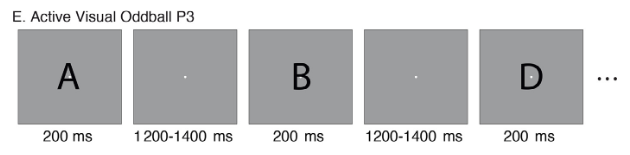
\includegraphics[width=0.8\textwidth]{eeg_visual_oddball.png}
  \caption{Experiment stimuli timeline: each letter is shown for 200ms followed by a 1200-1400ms break.}
  \label{fig:visual_oddball}
\end{figure}

\section{Preprocessing}
\label{sec:preprocessing}
As cleaned data of all subjects is already provided, the following section only focuses on the subjects $C = {S_{10}, S_{20}, S_{30}}$ for cleaning, re-referencing and the independent component analysis (ICA).
Because there was no examination of the data beforehand, the selection $C$ can be considered random.


\subsection{Cleaning}
The purpose of cleaning is to remove bad segments of the recordings, bad channels and in the worst case also bad subjects.
Criteria for removal are noisy, missing or extreme data values.
Extreme data can occur due to measurement errors like changes in the electrode-scalp conductivity during the experiment.
The Python library mne provides a graphical user interface to explore the data for each subject and annotate bad segments.
This GUI can be called with the plot() method in combination with \%matplotlib qt.

\subsubsection{Subject 10}
During the cleaning of subject $S_{10}$ 7 segments of heavy noise occurred during experiments.
These were marked as bad segments using the annotation feature of the interactive plot() function. 
The channels C5 and FP1 start to show a lot of noise after $t=80s$ and are excluded from the data.
Furthermore, the channels FP2 and F7 show high voltages which may be caused due to sub-optimal electrode-scalp activity and are therefore also marked as bad channels.
The annotated cleaned subject $S_{10}$ is saved to /data/subject10 using the helper function writeRAW2BIDS().

\begin{figure}[tbh!] 
  \centering
     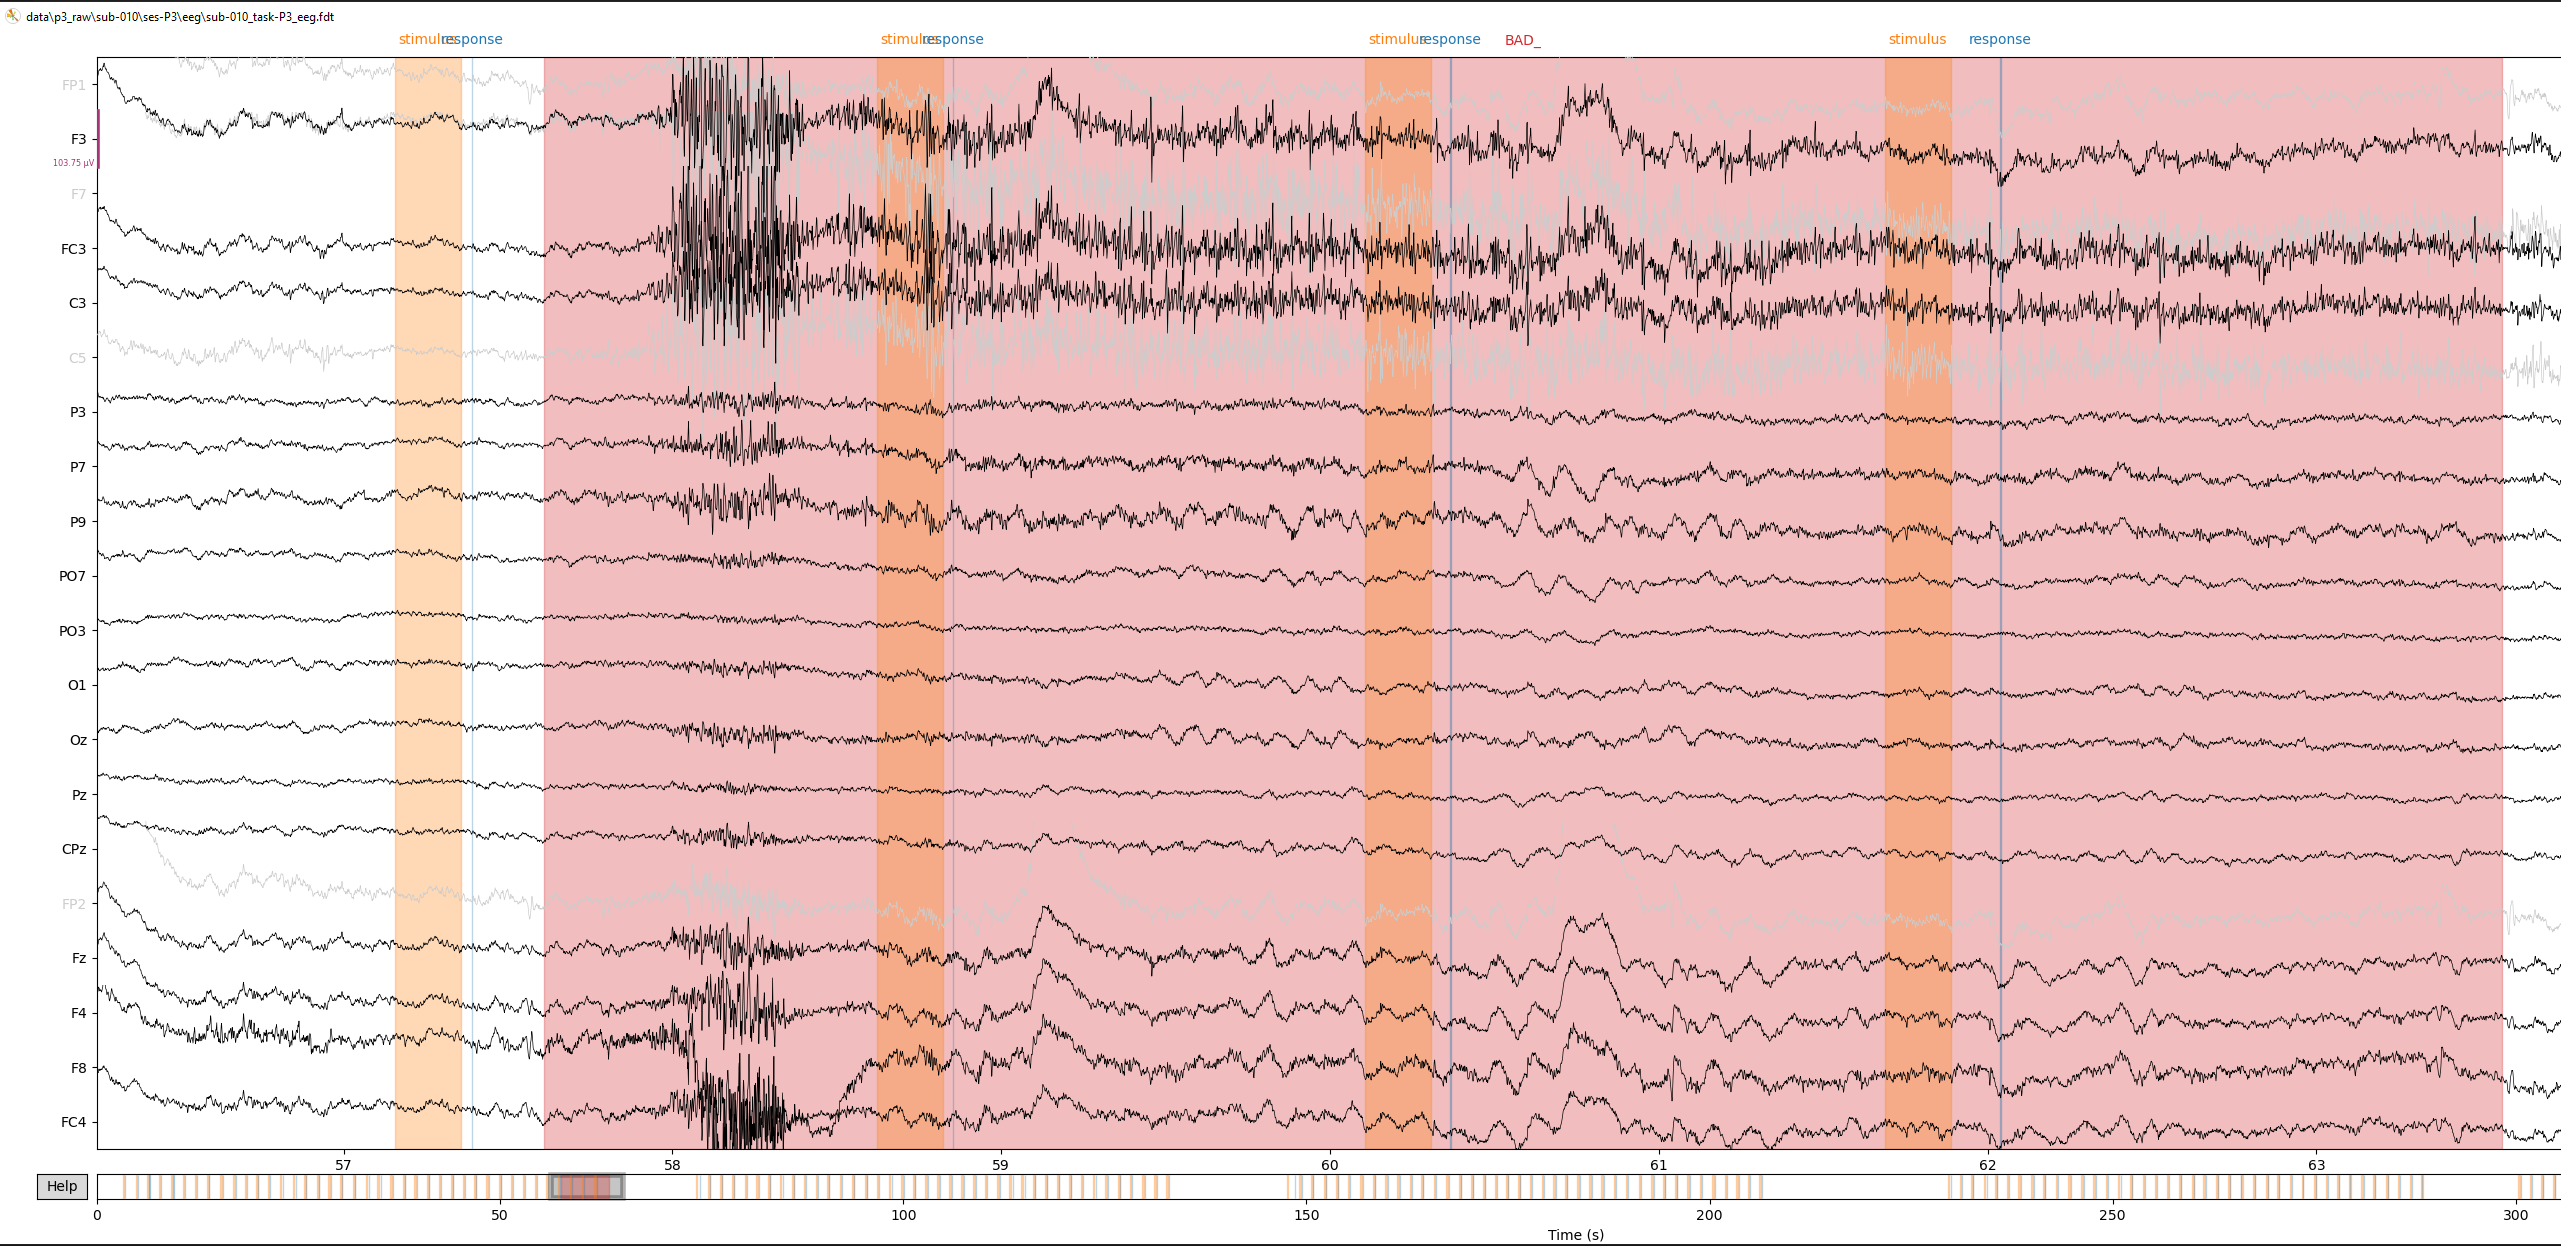
\includegraphics[width=0.8\textwidth]{eeg_clean_sub10.png}
  \caption{Noisy segment on multiple channels of $S_{10}$.}
  \label{fig:clean_sub10}
\end{figure}


\subsubsection{Subject 20}
Subject 20 shows the same unusually high voltages for the channels FP1 and FP2.
These are marked as bad channels.
There are 12 bad segments with noise during stimuli which are marked in the annotations.
The annotations for each subject are saved in the events.tsv file in /data/subject using again the helper function.

\subsubsection{Subject 30}
The EEG channels of $S_{30}$ show significantly higher amplitudes compared to $S_{10}$ and $S_{20}$.
To be able to see all amplitudes of the channels the y-axis scaling has to be set to more than 300\textmu v with an unchanged x-axis scaling of 1s.
Additionally, subject 30 shows 6 channels with a lot of noise over the entire experiment duration.
The channels FP1, P7, PO7, FP2, F4 and F8 are therefore marked as bad channels.
\begin{figure}[tbh!] 
  \centering
     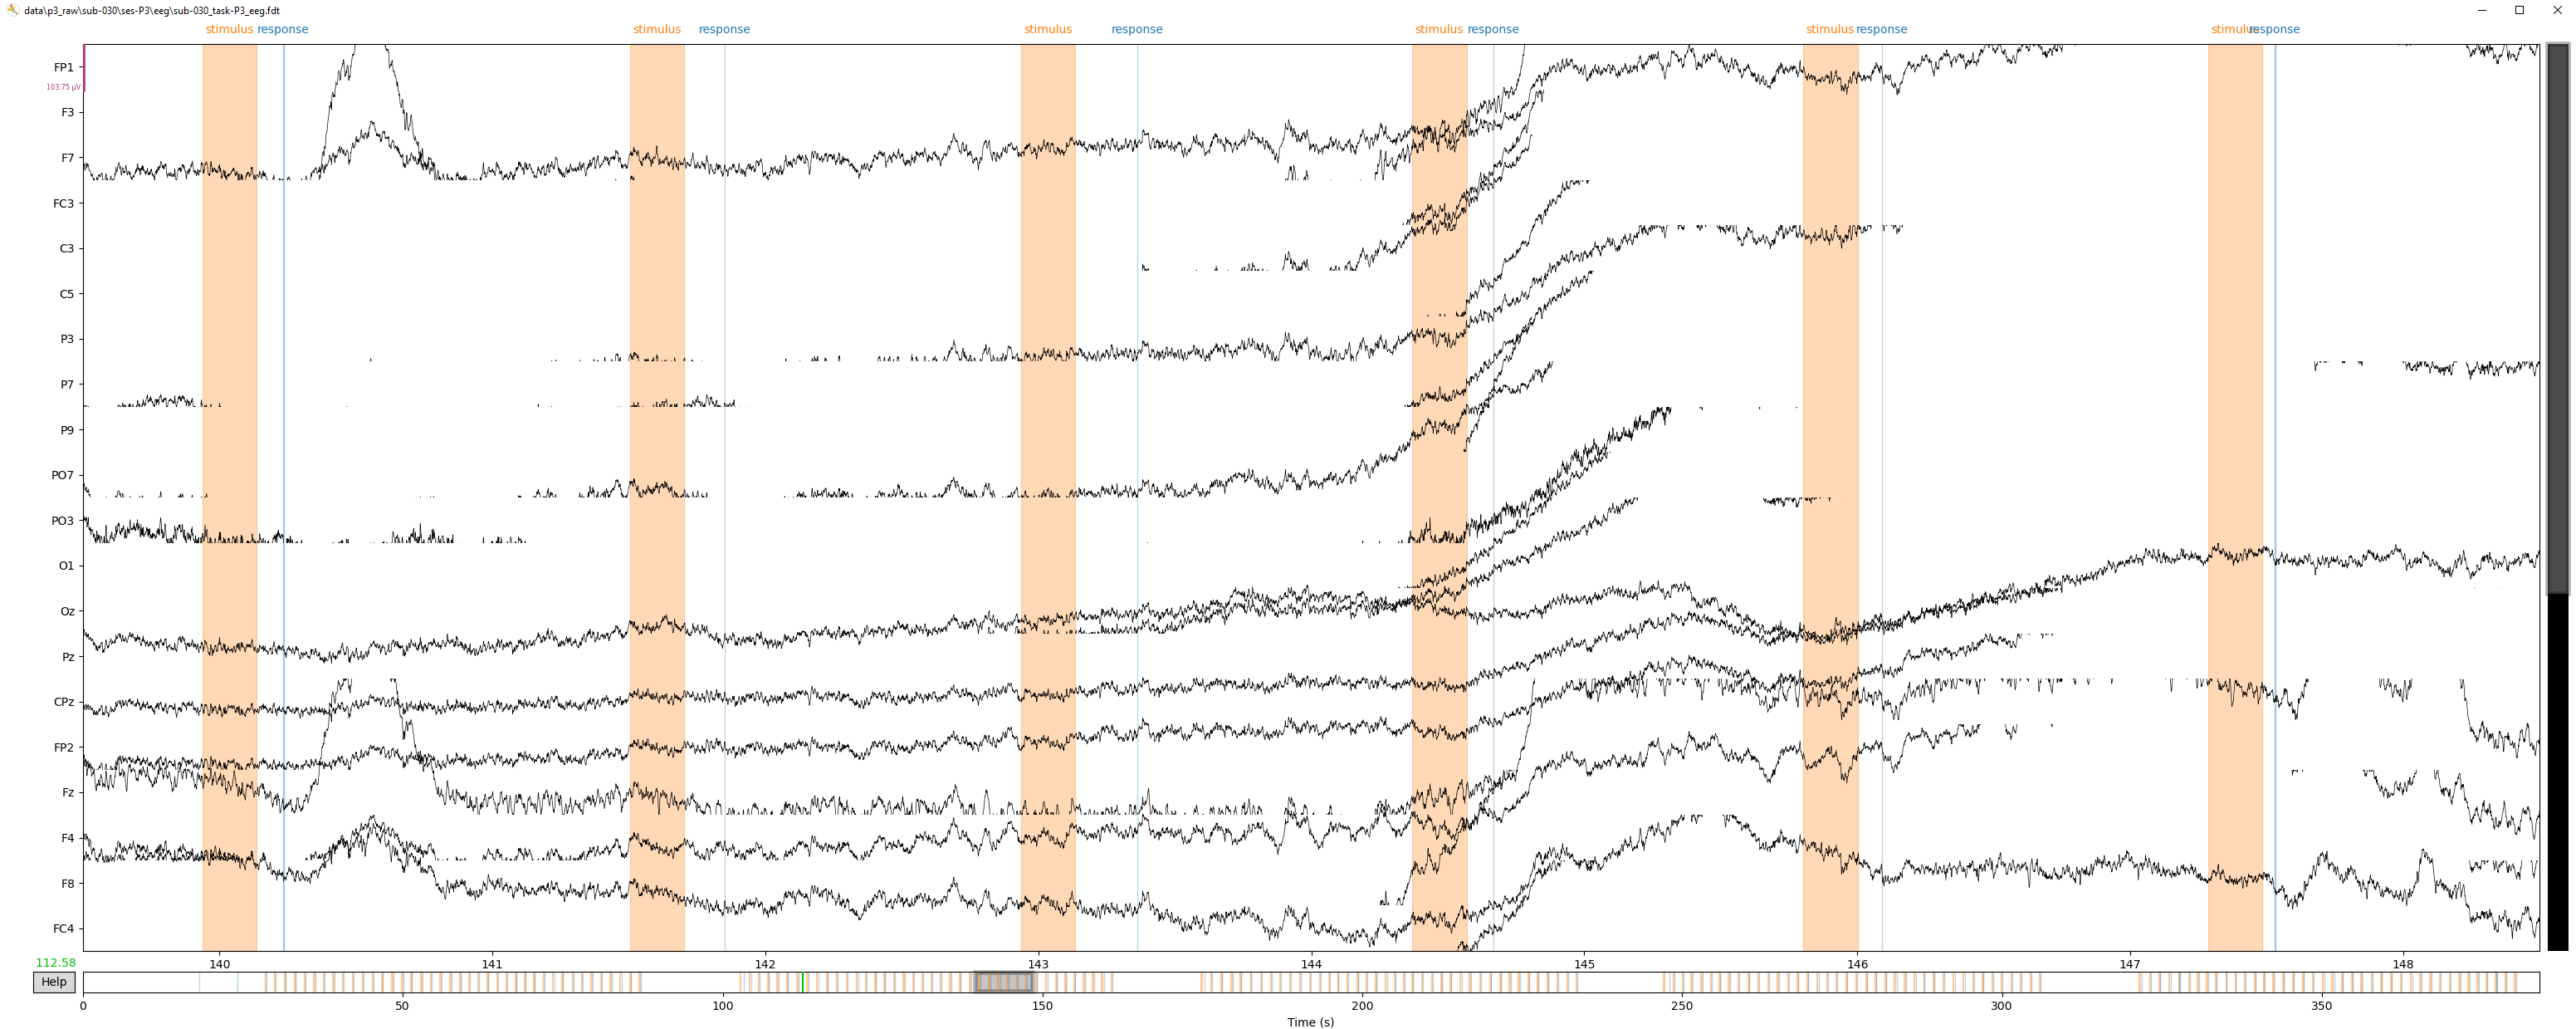
\includegraphics[width=0.8\textwidth]{eeg_clean_sub30.png}
  \caption{High voltages for most of the channels of $S_{30}$. The x-axis scaling is set to 103.75\textmu v}
  \label{fig:clean_sub10}
\end{figure}

\subsection{Re-referencing}
Re-referencing ensures that outside signals are removed and the data baseline is corrected by this outside noise.
\caay{Yao2019} describe different techniques for reference selection, such as single channel references (physical reference), linked mastoids or average reference (virtual reference).
The physical reference is the electrode placed at the top of the scalp (e.g. Cz, Fz, Oz) during online recording\pcaay{Hu2019}.
For this project the physical reference channel Fz was set as reference.
The Python mne library provides the function set\_eeg\_reference() to specify reference channels, which is applied for the subjects in $C = {S_{10}, S_{20}, S_{30}}$.

\subsection{Filtering}
EEG signals are prone to two different types of noise.
Low frequencies lead to slow and long-time drifts in EEG signal values, which can distort peak values between different epochs.
These slow drifts can be caused by a change of physical conditions, for instance subjects sweating in small amounts which modifies the electrode-scalp conductivity.
Usually these drifts are caused by frequencies below 1Hz.
The second type of noise affecting EEG measurements is high frequency noise, caused by the power line of the EEG measurement system.
In the following section, lowpass and highpass filters are used to reduce both types of noises for all subjects $S_i$.

\begin{figure}[tbh!] 
  \centering
     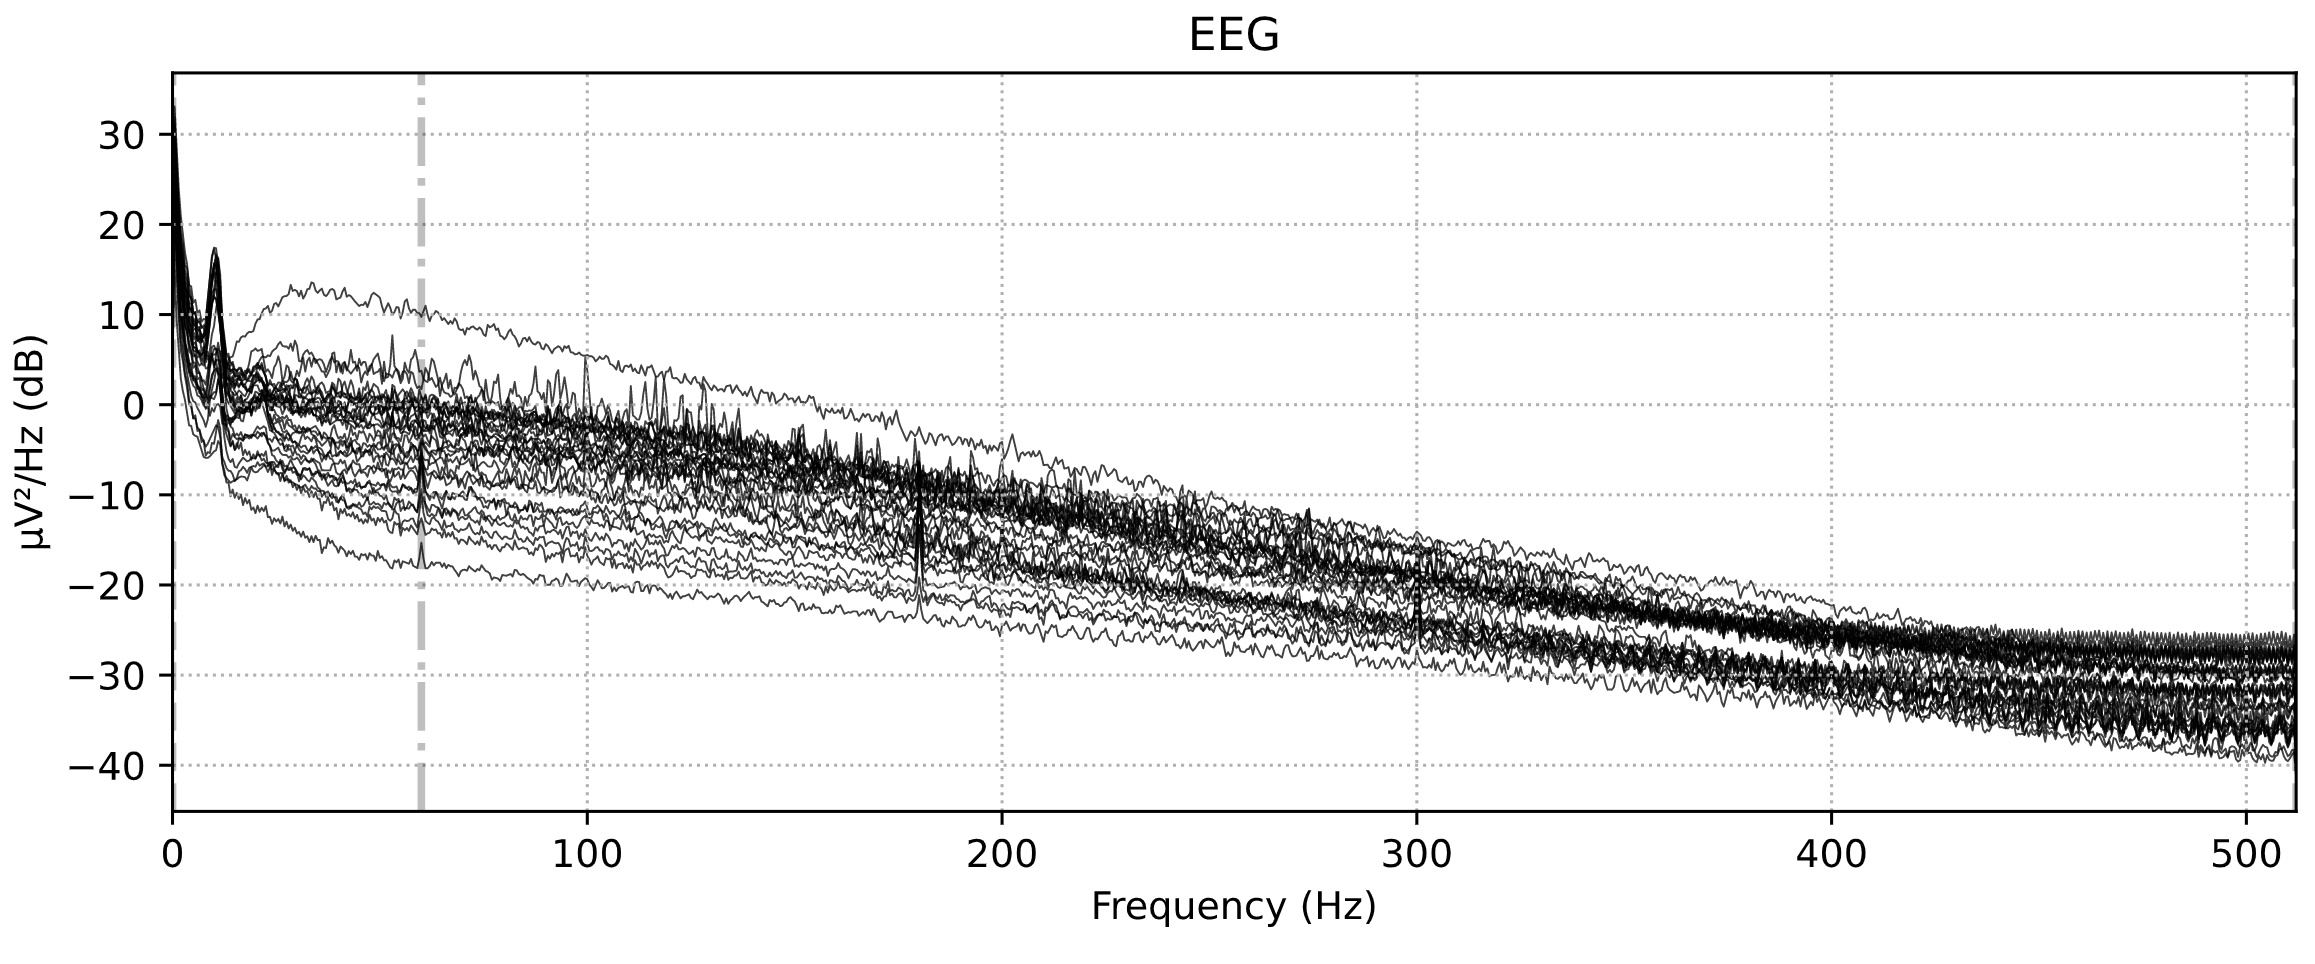
\includegraphics[width=0.8\textwidth]{eeg_psd.png}
  \caption{Power spectrum of the signal data of $S_1$ on all channels visualized using the mne function plot\_psd()}
  \label{fig:eeg_psd}
\end{figure}

\subsubsection{Highpass filter application}
To find the optimal cutoff frequency for the highpass filter 8 different frequencies are plotted using plot\_psd() 
($F={0.05, 0.1, 0.2, 0.3, 0.4, 0.6, 0.7}$).
Figure~\ref{fig:filteringHighpassComparison} showcases the effect of a 0.05Hz and 0.7Hz highpass filter cutoff frequency.
At 0.7Hz the filter is very effective in removing the unwanted slow drifts from the data. 

\begin{figure}[tbh!] 
\centering
 \begin{subfigure}[t]{0.5\textwidth}
        \centering
        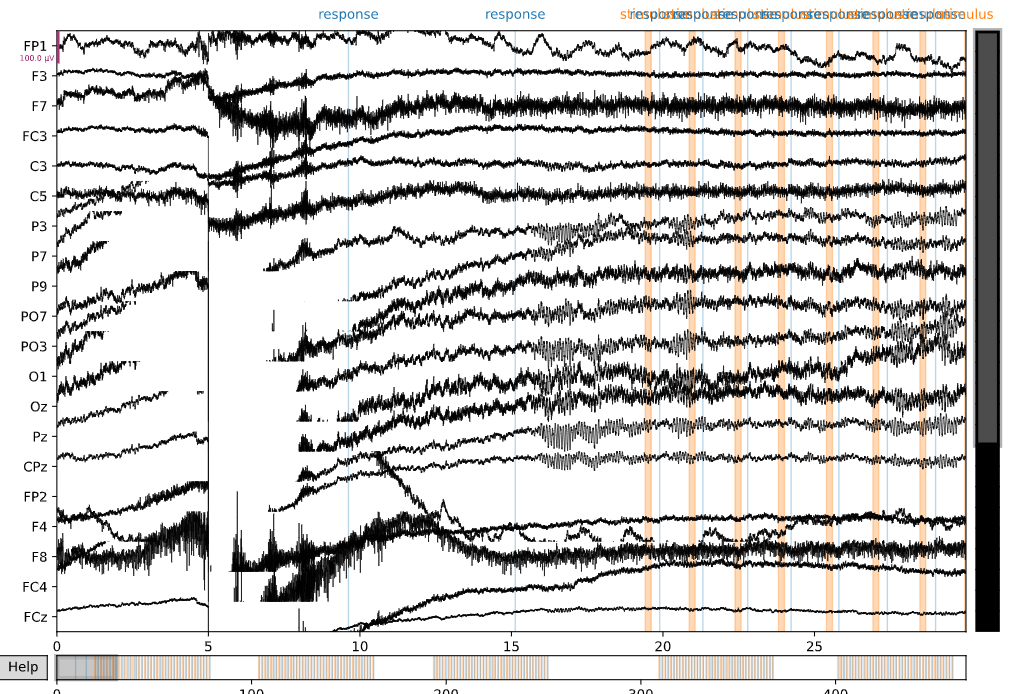
\includegraphics[height=2.0in]{hp005.png}
\caption{EEG of $S_1$ after the application of a highpass filter with a cutoff frequency of F[0]=0.05Hz}
\end{subfigure}%
    ~ 
\begin{subfigure}[t]{0.5\textwidth}
        \centering
        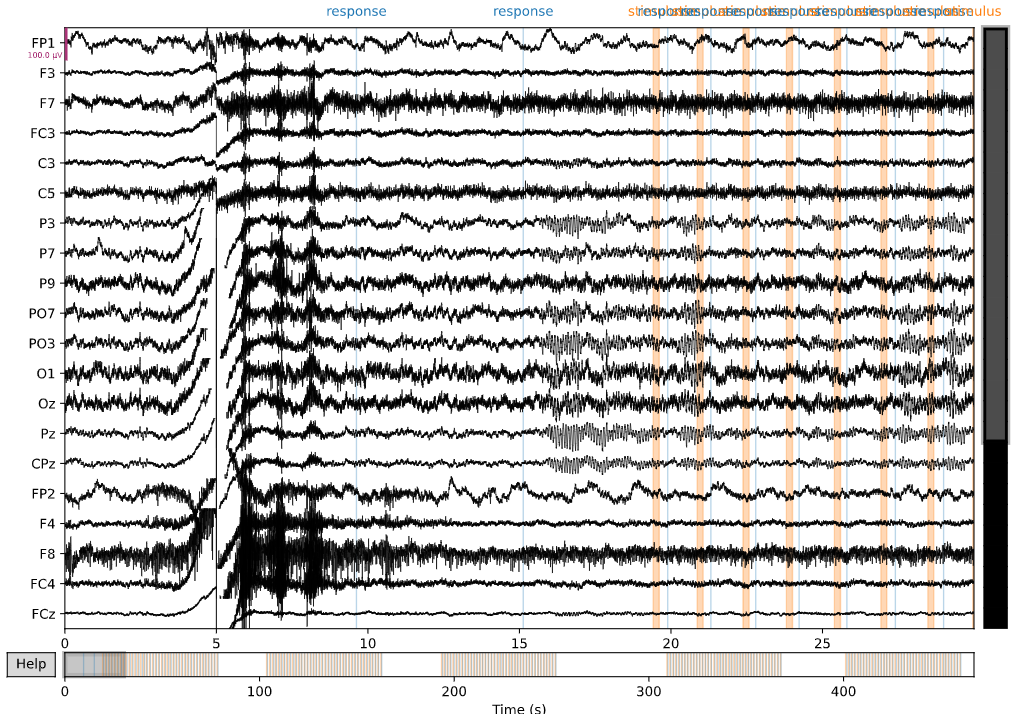
\includegraphics[height=2.0in]{hp07.png}
        \caption{EEG of $S_1$ after the application of a highpass filter with a cutoff frequency of F[6]=0.7Hz}
\end{subfigure}
    \caption{Comparison of effects on slow long-term signal drifts using different highpass filter cutoff frequencies. After application of the 0.7Hz highpass filter all slow drifts disappeared.}
    \label{fig:filteringHighpassComparison}
\end{figure}

\begin{figure}[tbh!] 
\centering
 \begin{subfigure}[t]{0.5\textwidth}
        \centering
        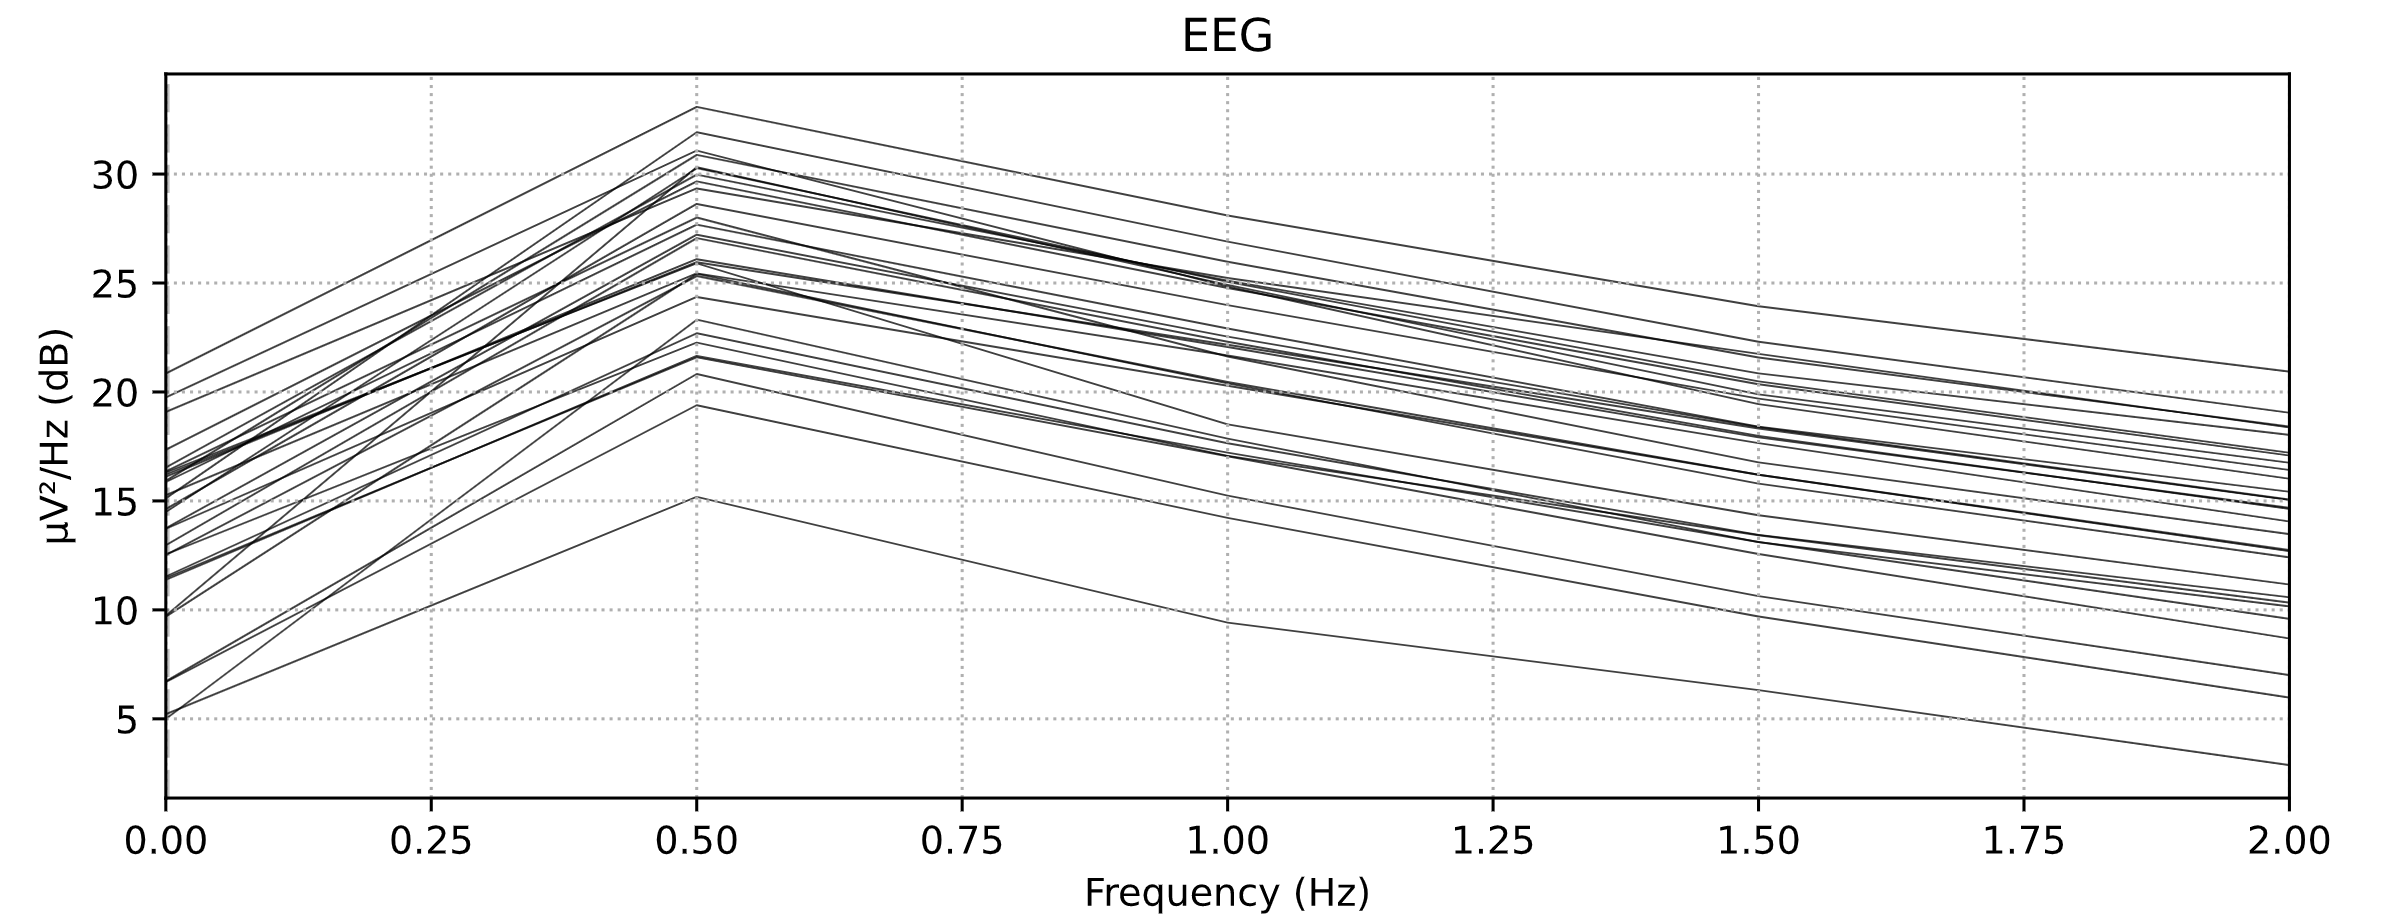
\includegraphics[height=1.3in]{highpassBefore.png}
\caption{Unfiltered powerspectrum of $S_1$.}
\end{subfigure}%
    ~ 
\begin{subfigure}[t]{0.5\textwidth}
        \centering
        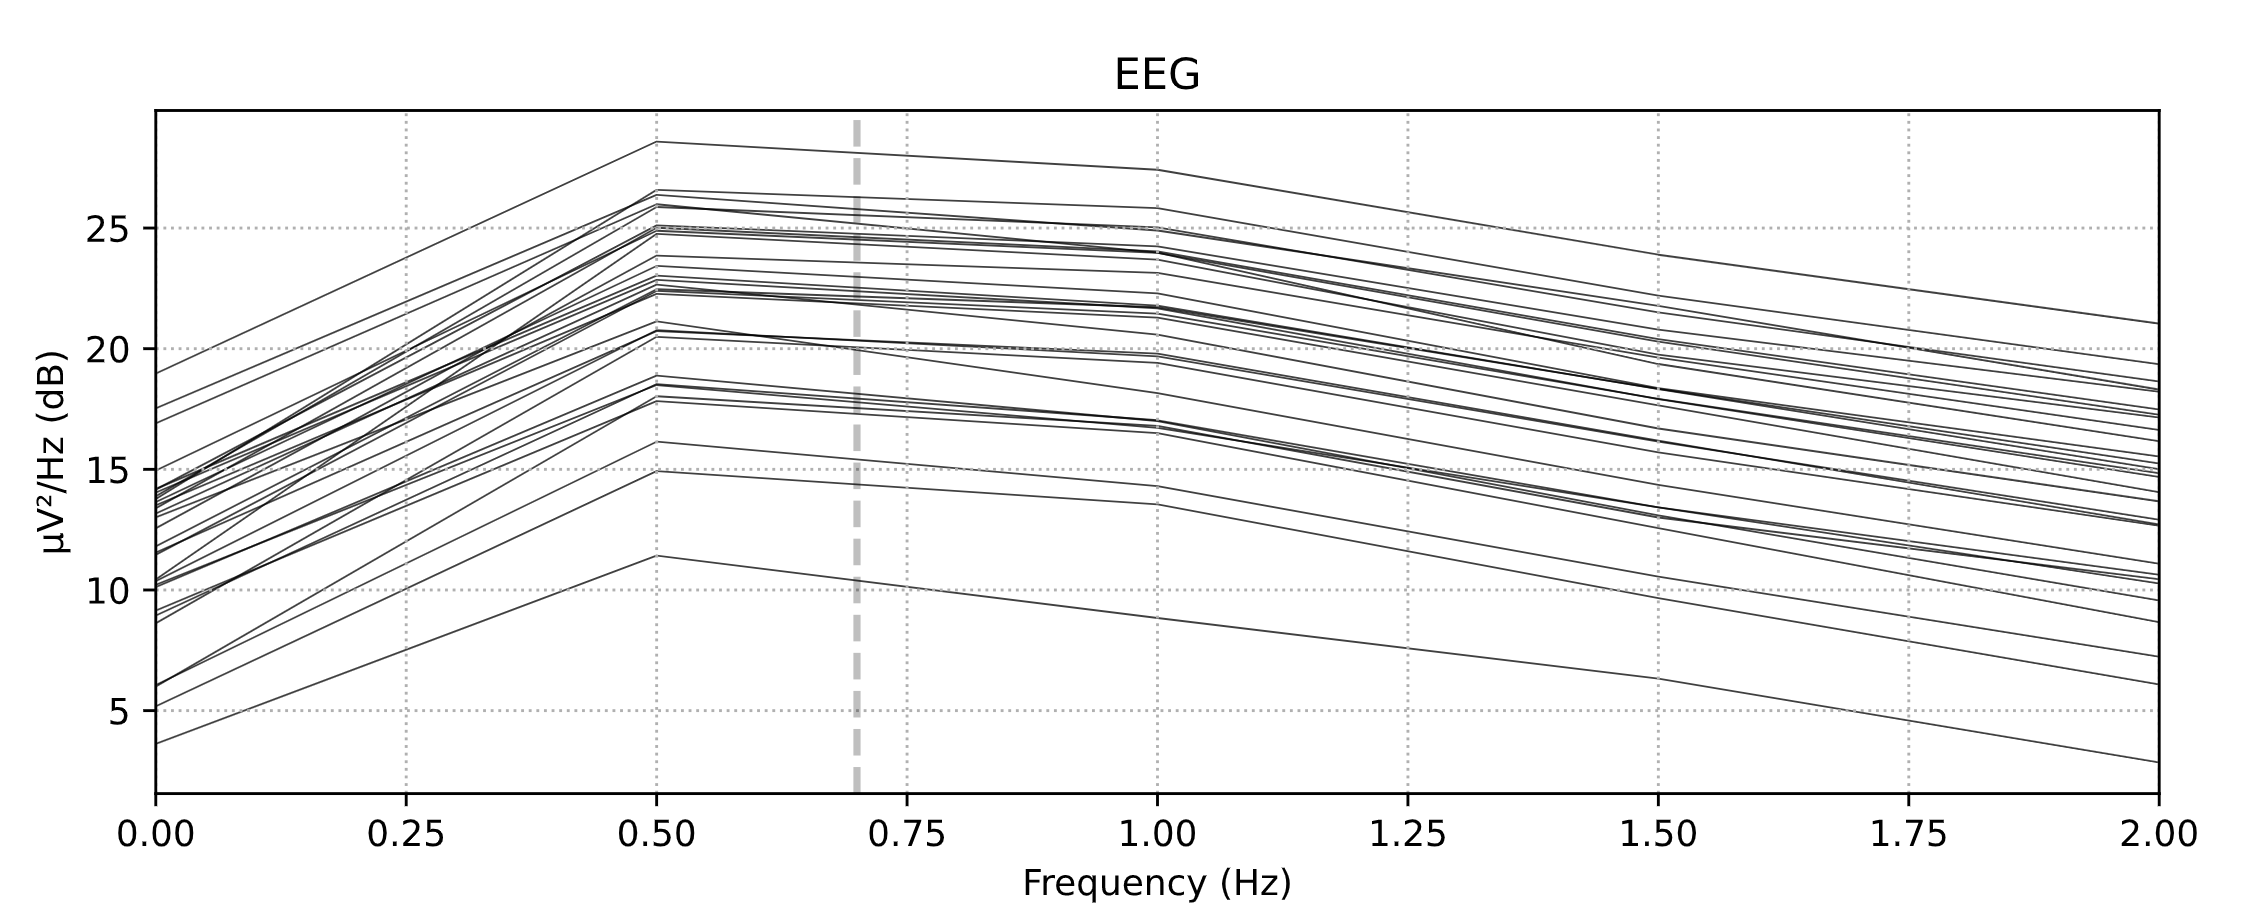
\includegraphics[height=1.3in]{highpassAfter.png}
        \caption{Filtered powerspectrum of $S_1$ after the application of a highpass filter with a cutoff frequency of F[0]=0.7Hz}
\end{subfigure}
    \caption{After filtering low frequency amplitudes below 1.5Hz drop, which can be seen by a decrease of y-axis scaling from 30 to 25.}
    \label{fig:filteringHighpassComparisonApplied}
\end{figure}

After the application of the 0.7Hz filter the powerspectrum indeed shows a significant decrease in amplitude for low frequencies as shown in figure ~\ref{fig:filteringHighpassComparisonApplied}.
Therefore, the 0.7Hz highpass filter frequency is found to be adequate and is used to filter the data of all subjects.


\subsubsection{Lowpass filter application}
To find the optimal cutoff frequency for the lowpass filter 5 different frequencies $F={40, 45, 50, 55, 60}$ are plotted using plot\_psd() to compare their impact on the data.
Figure~\ref{fig:filteringLowpassComparison} showcases the effect of a 45Hz and 60Hz lowpass filter cutoff frequency.
At 45Hz the filter is most effective in removing the unwanted power noise from the data.

\begin{figure}[tbh!] 
\centering
 \begin{subfigure}[t]{0.5\textwidth}
        \centering
        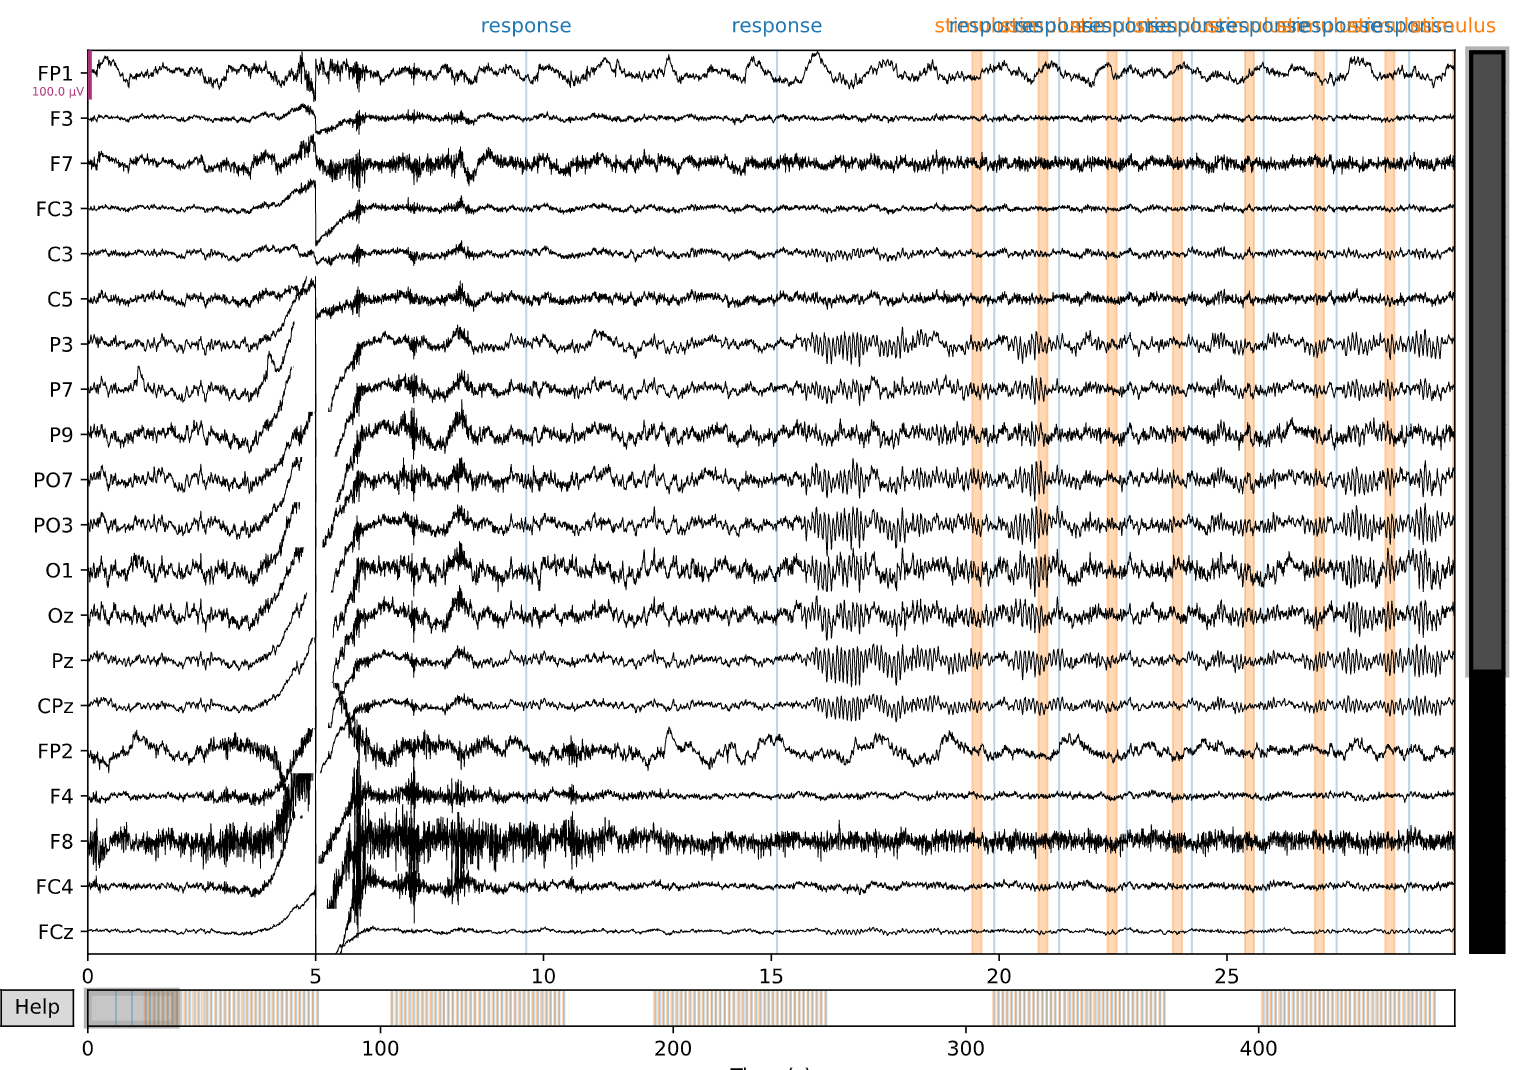
\includegraphics[height=2.0in]{lp60.png}
\caption{EEG of $S_1$ after the application of a highpass filter with a cutoff frequency of 0.7Hz and a lowpass filter cutoff frequency 60Hz.}
\end{subfigure}%
    ~ 
\begin{subfigure}[t]{0.5\textwidth}
        \centering
        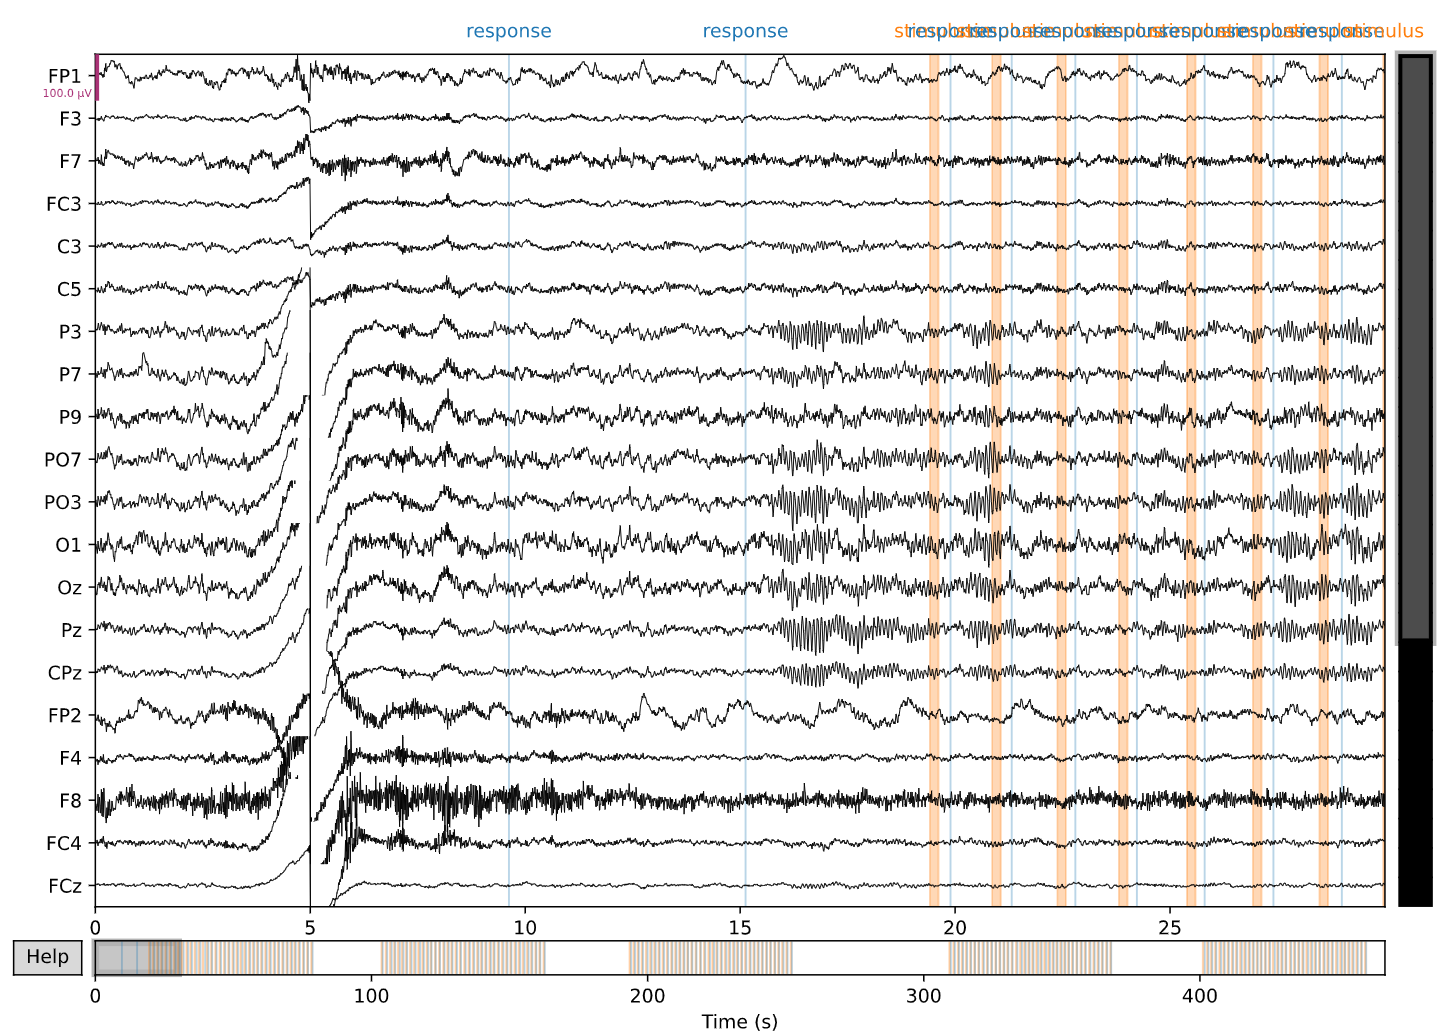
\includegraphics[height=2.0in]{lp45.png}
        \caption{EEG of $S_1$ after the application of a highpass filter with a cutoff frequency of 0.7Hz and a lowpass filter cutoff frequency 45Hz. The noise removal effect can be seen best for channel F7.}
\end{subfigure}
    \caption{Comparison of effects on power noise using different lowpass filter cutoff frequencies.}
    \label{fig:filteringLowpassComparison}
\end{figure}

\begin{figure}[tbh!] 
\centering
 \begin{subfigure}[t]{0.5\textwidth}
        \centering
        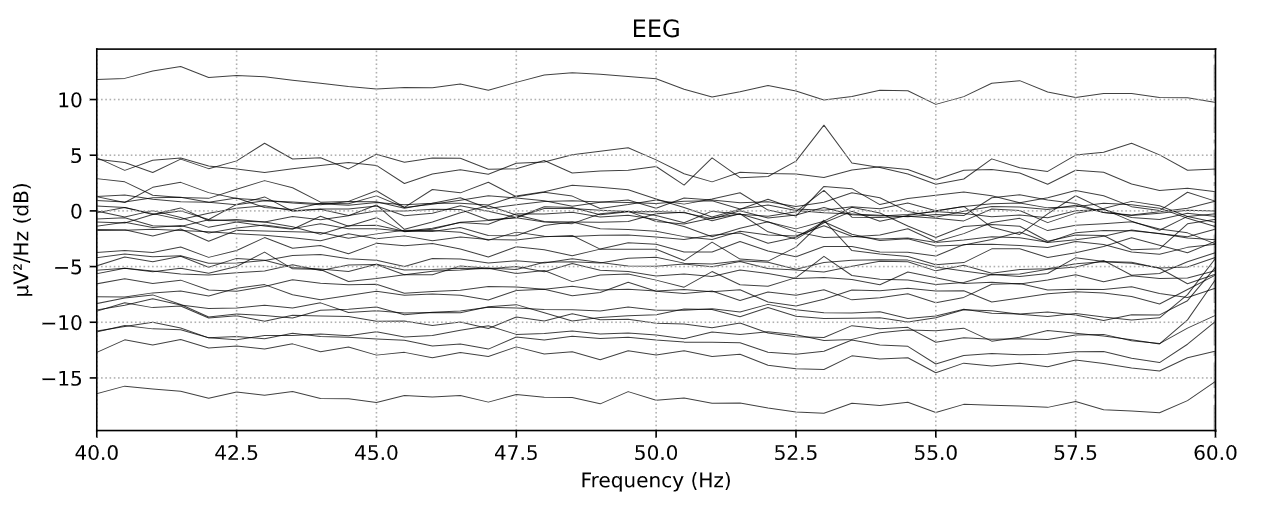
\includegraphics[height=1.3in]{lowpassBefore.png}
\caption{Powerspectrum of $S_1$ filtered with a 0.7Hz highpass filter.}
\end{subfigure}%
    ~ 
\begin{subfigure}[t]{0.5\textwidth}
        \centering
        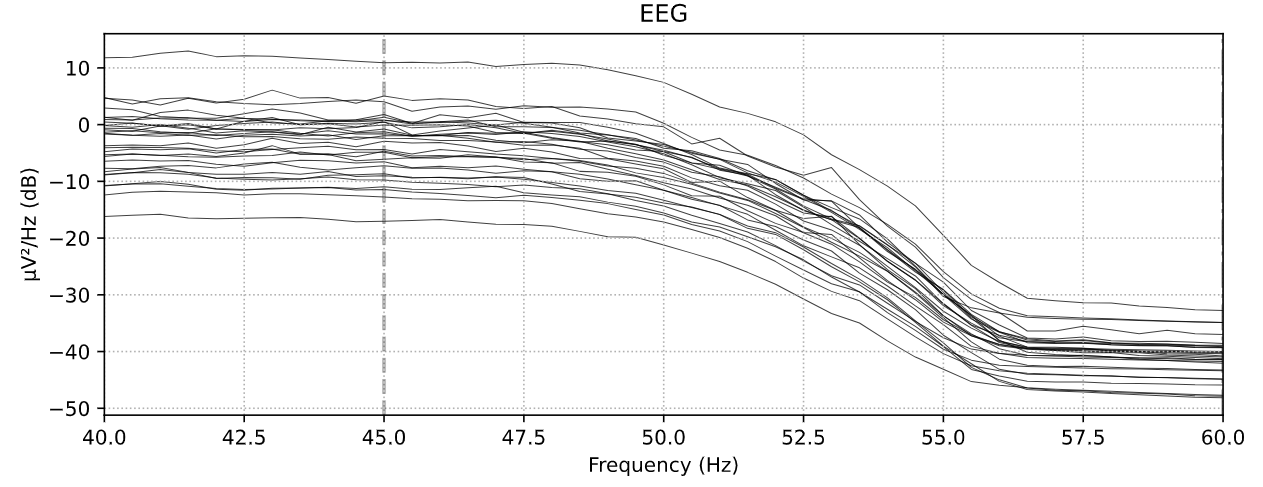
\includegraphics[height=1.3in]{lowpassAfter.png}
        \caption{Filtered powerspectrum of $S_1$ after the application of a highpass filter with a cutoff frequency of 0.7Hz and a lowpass filter with a cutoff frequency of 45Hz}
\end{subfigure}
    \caption{After filtering the high frequency amplitudes above 45Hz drop and do not significantly contribute to the signal anymore.}
    \label{fig:filteringLowpassComparisonApplied}
\end{figure}

As the lowpass filter with a frequency of 45Hz shows promising results for noisy channels, this filter is applied to all subjects.
\FloatBarrier



\subsection{Independent component analysis}
The goal of independent component analysis (ICA) is to remove artifacts and noise from the data.
However when the data is presented per channel this artifact detection is not trivial.
The independent components responsible for the EEG channel amplitudes can be extracted.
For instance eye blinks cause a lot of disturbance on multiple channels.
The idea is to extract all independent components of the signal and visually map them to the subjects brain.
In this way, specific noisy components can be identified and excluded.
After this selection, the remaining components are recombined resulting in an artifact free signal.
In the following, ICA components for the subjects in $C = {S_{10}, S_{20}, S_{30}}$ are extracted, examined, labeled and recombined.

The website labeling.ucsd.edu offers a introduction course into labeling ICA components for EEG data\pcaay{pion-tonachini}.
This course was used as reference guideline to identify bad components.
Figure~\ref{fig:ica10Analysis} shows an example for a muscle artifact detection in the labeling course and in the EEG data of subject $S_{10}$.
All components of the subjects are shown in figure~\ref{fig:ica10}, ~\ref{fig:ica20} and~\ref{fig:ica30}.
Following the labeling guideline of the website \pcaay{pion-tonachini} the excluded components for the three subjects in $C$ are listed in table 1.

% Please add the following required packages to your document preamble:
% \usepackage[table,xcdraw]{xcolor}
% If you use beamer only pass "xcolor=table" option, i.e. \documentclass[xcolor=table]{beamer}
\begin{table}[]
\centering
\begin{tabular}{|l|l|l|}
\hline
\rowcolor[HTML]{9B9B9B} 
\multicolumn{1}{|c|}{\cellcolor[HTML]{9B9B9B}\textbf{Subject}} & \multicolumn{1}{c|}{\cellcolor[HTML]{9B9B9B}\textbf{ICA}} & \multicolumn{1}{c|}{\cellcolor[HTML]{9B9B9B}\textbf{Reason for exclusion}} \\ \hline
10                                                             & 000                                                       & Eye movement                                                               \\ \hline
10                                                             & 006                                                       & Muscle Artifact                                                            \\ \hline
10                                                             & 018                                                       & Other                                                                      \\ \hline
10                                                             & 019                                                       & Other                                                                      \\ \hline
10                                                             & 020                                                       & Other                                                                      \\ \hline
10                                                             & 021                                                       & Muscle Artifact                                                                      \\ \hline
20                                                             & 000                                                       & Exe movement                                                               \\ \hline
20                                                             & 002                                                       & Muscle Artifact                                                            \\ \hline
20                                                             & 009                                                       & Muscle Artifact                                                            \\ \hline
30                                                             & 000                                                       & Muscle Artifact                                                            \\ \hline
30                                                             & 001                                                       & Muscle Artifact                                                            \\ \hline
30                                                             & 002                                                       & Muscle Artifact                                                            \\ \hline
30                                                             & 008                                                       & Channel noise                                                              \\ \hline
30                                                             & 011                                                       & Channel noise                                                              \\ \hline
30                                                             & 021                                                       & Other                                                                      \\ \hline
\end{tabular}
\label{tab:icaExclude}
\caption{Excluded ICA components due to artifacts}
\end{table}

\begin{figure}[tbh!] 
\centering
 \begin{subfigure}[t]{0.5\textwidth}
        \centering
        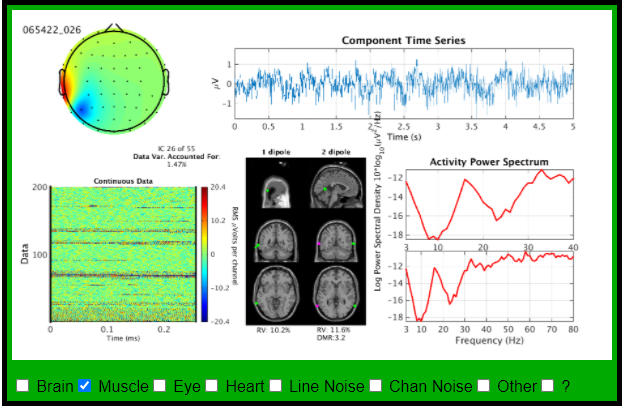
\includegraphics[height=2.0in]{ica10AnalysisLabel.png}
\caption{Ground truth label for a muscle artifact according to \caay{pion-tonachini}}
\end{subfigure}%
    ~ 
\begin{subfigure}[t]{0.5\textwidth}
        \centering
        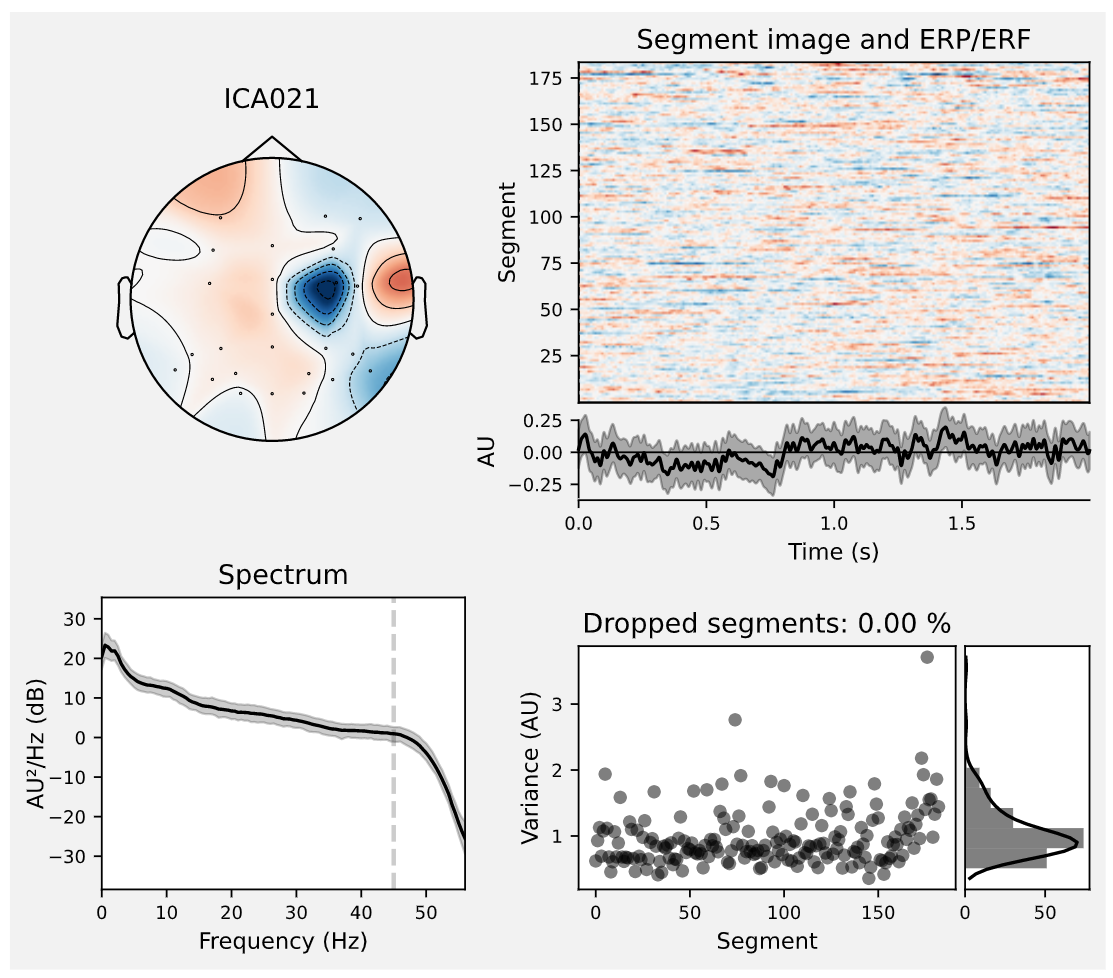
\includegraphics[height=2.0in]{ica10Analysis.png}
        \caption{Excluded muscle artifact ICA021 of $S_{10}$.}
\end{subfigure}
    \caption{Bad ICA component 21 of $S_{10}$ due to muscle activity at the subjects temples.}
     \label{fig:ica10Analysis}
\end{figure}


\begin{figure}[tbh!] 
  \centering
     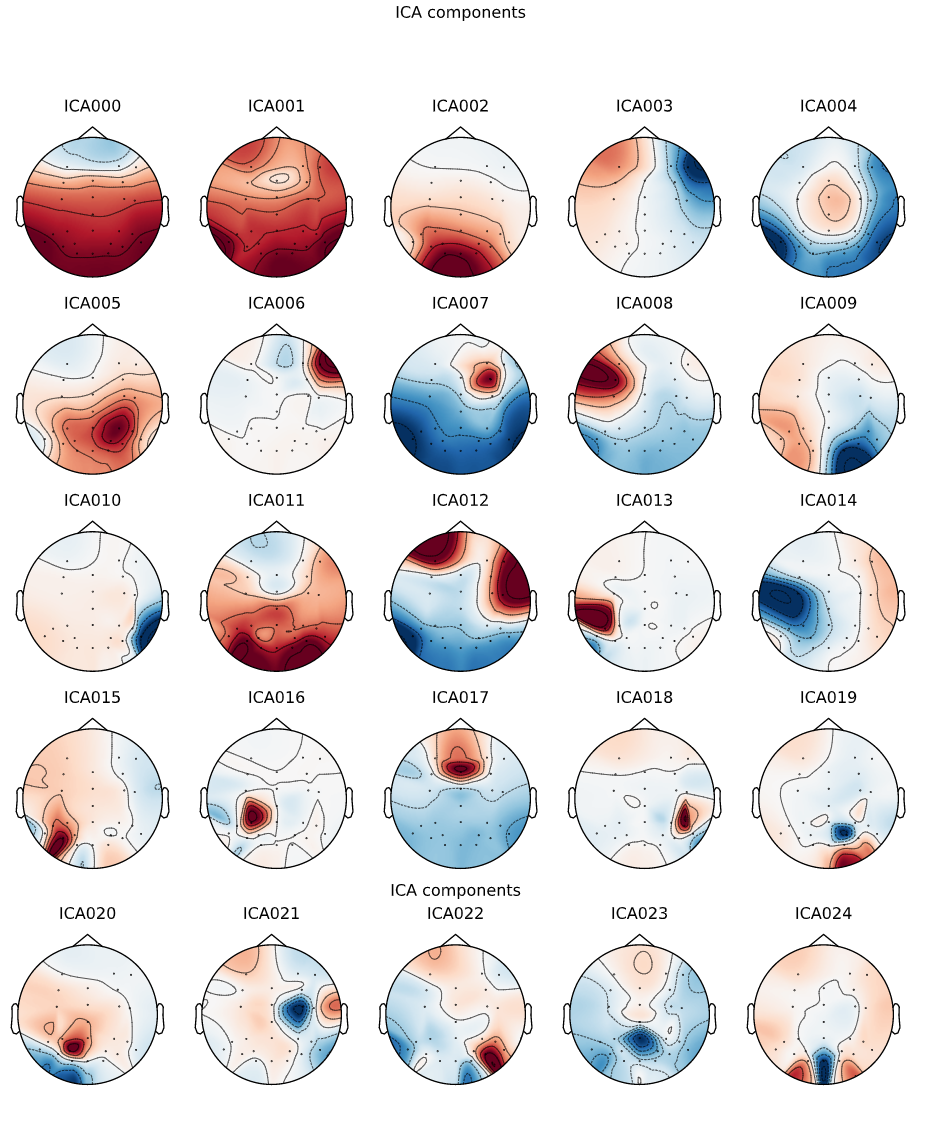
\includegraphics[width=0.8\textwidth]{ica10.png}
  \caption{ICA components of $S_{10}$.}
  \label{fig:ica10}
\end{figure}

\begin{figure}[tbh!] 
  \centering
     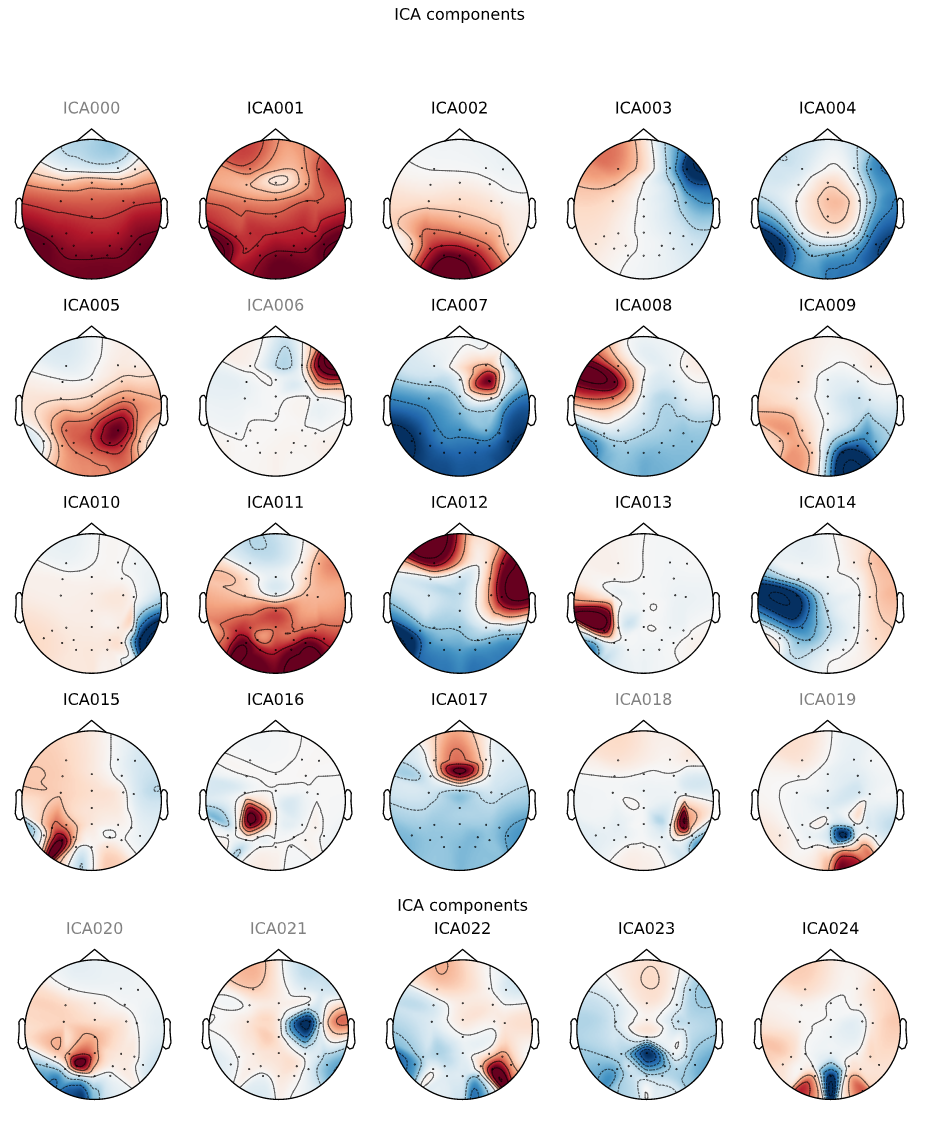
\includegraphics[width=0.8\textwidth]{ica20.png}
  \caption{ICA components of $S_{20}$. Excluded components are labeled in gray.}
  \label{fig:ica20}
\end{figure}

\begin{figure}[tbh!] 
  \centering
     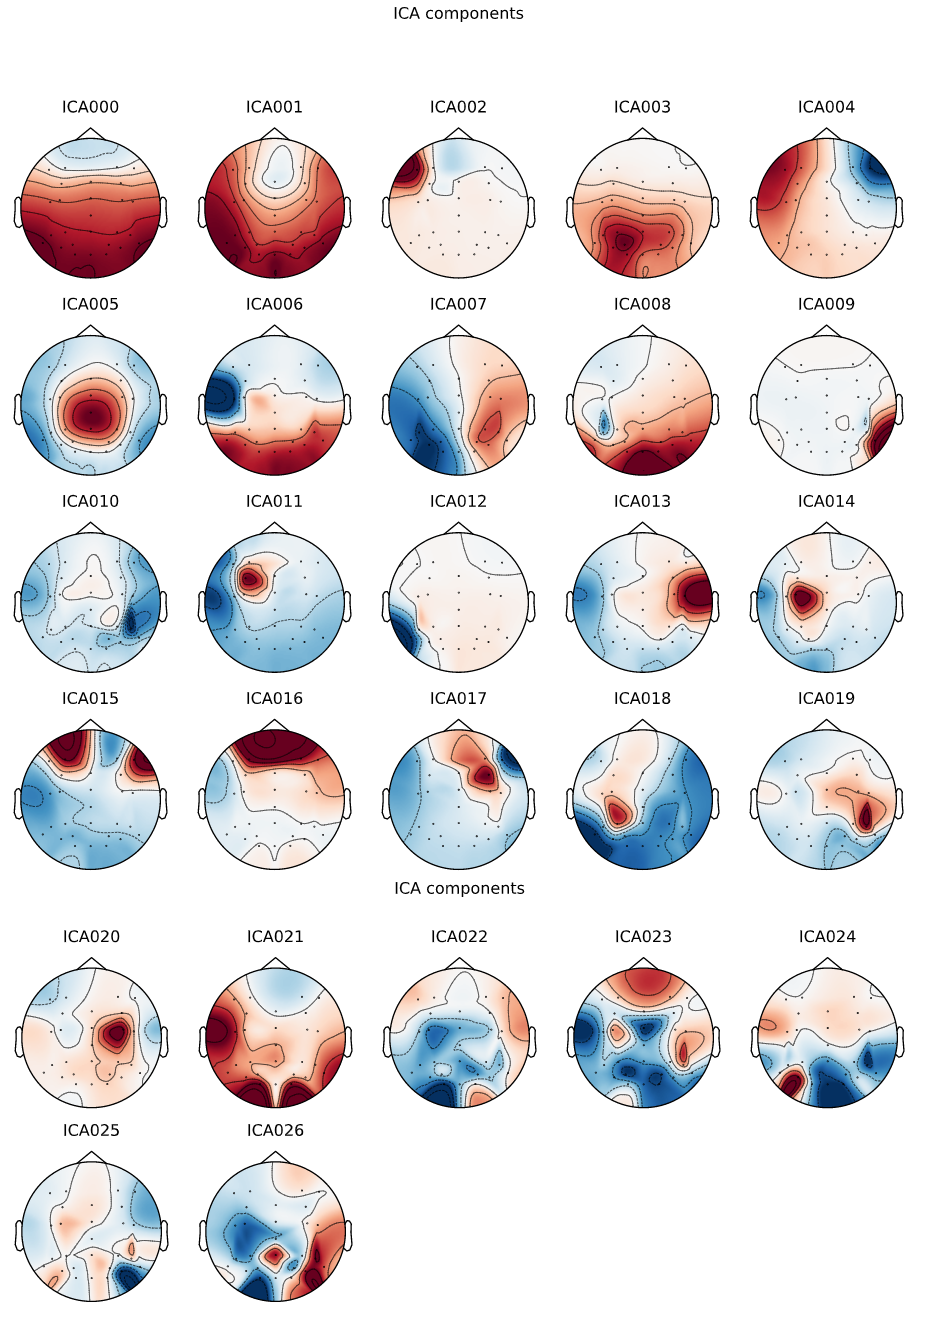
\includegraphics[width=0.8\textwidth]{ica30.png}
  \caption{ICA components of $S_{30}$.}
  \label{fig:ica30}
\end{figure}

\FloatBarrier

\section{ERP peak analysis}
\label{sec:erp}

\subsection{ERP extraction}
For the ERP peak analysis cleaned data of all 40 subjects is already provided.
The precomputed cleaned data contains information about bad channels, bad segments, and bad ICA components.
To load the provided precomputed data the functions load\textunderscore precomputed\textunderscore ica() and load\textunderscore precomputed\textunderscore badData() from ccs\textunderscore eeg\textunderscore semesterproject.py are used.
After loading the precomputed data, bad channels are excluded, annotations for bad segments are added and bad ICA components are excluded.
As in section~\ref{sec:preprocessing} the Fz channel is set as reference channel using set\_eeg\_reference().
A lowpass filter with cutoff frequency 45Hz and a highpass filter with cutoff frequency 0.7Hz is applied to the loaded data.
Finally new event modifiers are introduced.
The original experiment has a different event label for each stimulus combination of trial stimuli and block targets, resulting in a total of 25 different event identifiers for the 5 letters.
The event labels for responses are labeled with correct ($id=201$) and incorrect ($id=202$).
For the following steps in the pipeline the new event identifiers only separate between target stimulus or distractor stimulus.
From the provided events, epochs are distracted using the time interval $t_{min}=-0.1s$ and $t_{max}=0.8s$ around the stimulus event.
Each epoch is labeled with a new label according to the stimulus shown: If the original stimulus event id modulo 11 is equal to 0, the target stimulus is shown and a label named \textit{target}, otherwise a \textit{distractor} letter is shown.
The response event id is discarded and not added to the epoch event id.
For each EEG channel in each epoch the peak amplitude value and the time point of the peak amplitude value are computed and saved in a pandas data frame, which is appended to the mne.eeg.info dictionary.

\begin{figure}[tbh!] 
\centering
 \begin{subfigure}[t]{0.5\textwidth}
        \centering
        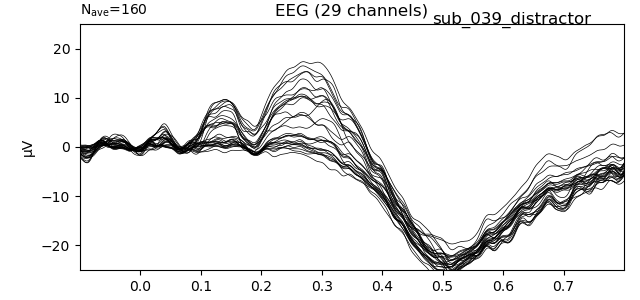
\includegraphics[height=1.3in]{sub039distractor.png}
	\caption{ERP averages of subject 39 for all good channels for $n=160$ epochs where a distractor stimuli was shown.}
\end{subfigure}%
    ~ 
\begin{subfigure}[t]{0.5\textwidth}
        \centering
        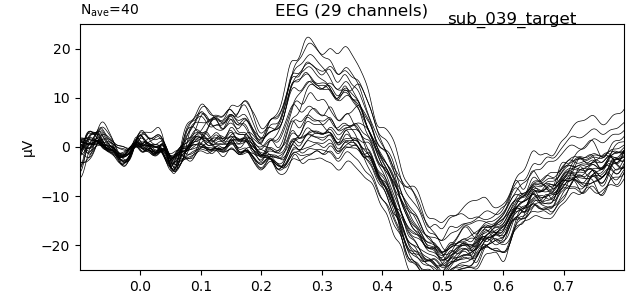
\includegraphics[height=1.3in]{sub039target.png}
        \caption{ERP averages of subject 39 for all good channels for $n=40$ epochs where the block target stimulus was shown.}
\end{subfigure}
    \caption{Comparison of ERP averages using all available epochs of the conditions \textit{target} and \textit{distractor} for $S_{39}$.}
     \label{fig:erpPeakAnalysis}
\end{figure}

\subsection{ERP peak analysis}
%~\ref{tab:erpPeaks39} 
Table 2 shows extracted ERP peak data for the subject 39.
For each channel the $tp$ time is the point in time in ms after the target stimulus where this channel ERP average peaks.
Most of the target peaks take place close before 300ms after the stimulus for this subject.
$tp$ value is the maximum value of each channels average of epochs where a target stimulus was shown.
The same concept is valid for the distractor stimuli, where $dp$ time is the timepoint of the peak value and $dp$ value the maximum value of the averaged epochs of this channel and subject if a distractor stimulus was shown.
The channels are sorted in descending order by the percentage of peak value increase from distractor stimulus to target stimulus.
For example the Cz channel average ERP peak for epochs where a target stimuli was shown is 70.7\% higher than the average ERP peak where a distractor stimulus was shown.
All channels except the P10 channel shown an increase in peak value when the target is shown.

This ERP peak value increase caused by target stimuli is statistically tested for each channel.
The ERP peak value increase for target stimuli of each channel is tested for a significance level of $\sigma=0.05$.
Therefore, for each channel the ERP peak values for each subject and for target stimuli and distractor stimuli epochs are collected in a list.
Each channel is tested with two lists, a target list and a distractor list.
The target list of this channel contains all ERP average peak values from epochs where a target stimlu was shown for all subjects.
The distractor list of this channel contains all ERP average peak values from epochs where a distractor stimuli was shown for this channel for all subjects.

% Please add the following required packages to your document preamble:
% \usepackage[table,xcdraw]{xcolor}
% If you use beamer only pass "xcolor=table" option, i.e. \documentclass[xcolor=table]{beamer}
\begin{table}[]
\centering
\begin{tabular}{|l|l|l|l|l|l|}
\hline
\rowcolor[HTML]{9B9B9B} 
\textbf{channel} & \textbf{$tp$ time in ms} & \textbf{$tp$ value in \textmu v} & \textbf{$dp$ time in ms} & \textbf{$dp$ value in \textmu v} & \textbf{increase in \%} \\ \hline
Cz               & 371                         & 4.88                         & 246                             & 1.43                             & 70.70\%                        \\ \hline
FCz              & 367                         & 1.81                         & -64                             & 0.65                             & 64.09\%                        \\ \hline
C3               & 323                         & 5.67                         & 251                             & 2.32                             & 59.08\%                        \\ \hline
FC3              & 287                         & 2.51                         & -64                             & 1.04                             & 58.57\%                        \\ \hline
F7               & 286                         & 3.90                         & 160                             & 1.63                             & 58.21\%                        \\ \hline
FP1              & 101                         & 2.87                         & -63                             & 1.30                             & 54.70\%                        \\ \hline
C5               & 285                         & 6.05                         & 272                             & 2.78                             & 54.05\%                        \\ \hline
F3               & 100                         & 2.27                         & -63                             & 1.18                             & 48.02\%                        \\ \hline
P3               & 286                         & 17.27                        & 278                             & 10.02                            & 41.98\%                        \\ \hline
F4               & 156                         & 1.39                         & 47                              & 0.94                             & 32.37\%                        \\ \hline
PO3              & 286                         & 22.33                        & 283                             & 15.29                            & 31.53\%                        \\ \hline
CPz              & 371                         & 8.41                         & 311                             & 5.76                             & 31.51\%                        \\ \hline
Pz               & 323                         & 12.99                        & 317                             & 9.67                             & 25.56\%                        \\ \hline
FP2              & -97                         & 1.84                         & 18                              & 1.37                             & 25.54\%                        \\ \hline
F8               & -85                         & 1.98                         & 134                             & 1.51                             & 23.74\%                        \\ \hline
C4               & 355                         & 3.60                         & 252                             & 2.77                             & 23.06\%                        \\ \hline
P4               & 291                         & 13.41                        & 309                             & 10.48                            & 21.85\%                        \\ \hline
C6               & 292                         & 3.32                         & 136                             & 2.61                             & 21.39\%                        \\ \hline
FC4              & 355                         & 1.36                         & 47                              & 1.07                             & 21.32\%                        \\ \hline
O1               & 283                         & 15.16                        & 279                             & 12.08                            & 20.32\%                        \\ \hline
P7               & 288                         & 13.31                        & 275                             & 10.76                            & 19.16\%                        \\ \hline
Oz               & 284                         & 14.84                        & 308                             & 12.06                            & 18.73\%                        \\ \hline
PO7              & 287                         & 16.98                        & 278                             & 13.84                            & 18.49\%                        \\ \hline
P9               & 262                         & 8.62                         & 276                             & 7.04                             & 18.33\%                        \\ \hline
PO4              & 289                         & 21.11                        & 278                             & 17.34                            & 17.86\%                        \\ \hline
PO8              & 290                         & 18.78                        & 277                             & 16.49                            & 12.19\%                        \\ \hline
P8               & 290                         & 11.04                        & 276                             & 10.33                            & 6.43\%                         \\ \hline
O2               & 288                         & 16.31                        & 283                             & 15.36                            & 5.82\%                         \\ \hline
P10              & 286                         & 6.51                         & 273                             & 6.59                             & -1.23\%                        \\ \hline
\end{tabular}
\label{tab:erpPeaks39}
\caption{Extracted average ERP peak values for all good channels for subject 39 for all epochs of the classes \textit{target}=$tp$ and \textit{distractor}=$dp$}
\end{table}

% Please add the following required packages to your document preamble:
% \usepackage[table,xcdraw]{xcolor}
% If you use beamer only pass "xcolor=table" option, i.e. \documentclass[xcolor=table]{beamer}
\begin{table}[]
\centering
\begin{tabular}{|r|r|}
\hline
\rowcolor[HTML]{9B9B9B} 
\multicolumn{1}{|c|}{\cellcolor[HTML]{9B9B9B}{\color[HTML]{000000} \textbf{channel}}} & \multicolumn{1}{c|}{\cellcolor[HTML]{9B9B9B}{\color[HTML]{000000} \textbf{p}}} \\ \hline
\rowcolor[HTML]{FFFFFF} 
{\color[HTML]{000000} \textbf{FCz}}                                                   & {\color[HTML]{000000} \textbf{0.01\%}}                                         \\ \hline
\rowcolor[HTML]{FFFFFF} 
{\color[HTML]{000000} \textbf{F4}}                                                    & {\color[HTML]{000000} \textbf{0.01\%}}                                         \\ \hline
\rowcolor[HTML]{FFFFFF} 
{\color[HTML]{000000} \textbf{F7}}                                                    & {\color[HTML]{000000} \textbf{0.04\%}}                                         \\ \hline
\rowcolor[HTML]{FFFFFF} 
{\color[HTML]{000000} \textbf{Cz}}                                                    & {\color[HTML]{000000} \textbf{0.14\%}}                                         \\ \hline
\rowcolor[HTML]{FFFFFF} 
{\color[HTML]{000000} \textbf{F3}}                                                    & {\color[HTML]{000000} \textbf{0.16\%}}                                         \\ \hline
\rowcolor[HTML]{FFFFFF} 
{\color[HTML]{000000} \textbf{F8}}                                                    & {\color[HTML]{000000} \textbf{0.20\%}}                                         \\ \hline
\rowcolor[HTML]{FFFFFF} 
{\color[HTML]{000000} \textbf{CPz}}                                                   & {\color[HTML]{000000} \textbf{0.44\%}}                                         \\ \hline
\rowcolor[HTML]{FFFFFF} 
{\color[HTML]{000000} \textbf{FC4}}                                                   & {\color[HTML]{000000} \textbf{0.46\%}}                                         \\ \hline
\rowcolor[HTML]{FFFFFF} 
{\color[HTML]{000000} \textbf{FP2}}                                                   & {\color[HTML]{000000} \textbf{0.64\%}}                                         \\ \hline
\rowcolor[HTML]{FFFFFF} 
{\color[HTML]{000000} \textbf{Pz}}                                                    & {\color[HTML]{000000} \textbf{0.82\%}}                                         \\ \hline
\rowcolor[HTML]{FFFFFF} 
{\color[HTML]{000000} \textbf{FP1}}                                                   & {\color[HTML]{000000} \textbf{1.01\%}}                                         \\ \hline
\rowcolor[HTML]{FFFFFF} 
{\color[HTML]{000000} \textbf{C4}}                                                    & {\color[HTML]{000000} \textbf{3.24\%}}                                         \\ \hline
\rowcolor[HTML]{FFFFFF} 
{\color[HTML]{000000} C3}                                                             & {\color[HTML]{000000} 5.19\%}                                                  \\ \hline
\rowcolor[HTML]{FFFFFF} 
{\color[HTML]{000000} FC3}                                                            & {\color[HTML]{000000} 9.17\%}                                                  \\ \hline
\rowcolor[HTML]{FFFFFF} 
{\color[HTML]{000000} P4}                                                             & {\color[HTML]{000000} 9.87\%}                                                  \\ \hline
\rowcolor[HTML]{FFFFFF} 
{\color[HTML]{000000} P3}                                                             & {\color[HTML]{000000} 11.91\%}                                                 \\ \hline
\rowcolor[HTML]{FFFFFF} 
{\color[HTML]{000000} C6}                                                             & {\color[HTML]{000000} 25.38\%}                                                 \\ \hline
\rowcolor[HTML]{FFFFFF} 
{\color[HTML]{000000} PO3}                                                            & {\color[HTML]{000000} 25.81\%}                                                 \\ \hline
\rowcolor[HTML]{FFFFFF} 
{\color[HTML]{000000} C5}                                                             & {\color[HTML]{000000} 33.30\%}                                                 \\ \hline
\rowcolor[HTML]{FFFFFF} 
{\color[HTML]{000000} PO4}                                                            & {\color[HTML]{000000} 38.00\%}                                                 \\ \hline
\rowcolor[HTML]{FFFFFF} 
{\color[HTML]{000000} PO8}                                                            & {\color[HTML]{000000} 56.78\%}                                                 \\ \hline
\rowcolor[HTML]{FFFFFF} 
{\color[HTML]{000000} P7}                                                             & {\color[HTML]{000000} 60.64\%}                                                 \\ \hline
\rowcolor[HTML]{FFFFFF} 
{\color[HTML]{000000} P10}                                                            & {\color[HTML]{000000} 62.30\%}                                                 \\ \hline
\rowcolor[HTML]{FFFFFF} 
{\color[HTML]{000000} PO7}                                                            & {\color[HTML]{000000} 64.21\%}                                                 \\ \hline
\rowcolor[HTML]{FFFFFF} 
{\color[HTML]{000000} O2}                                                             & {\color[HTML]{000000} 69.63\%}                                                 \\ \hline
\rowcolor[HTML]{FFFFFF} 
{\color[HTML]{000000} P8}                                                             & {\color[HTML]{000000} 70.81\%}                                                 \\ \hline
\rowcolor[HTML]{FFFFFF} 
{\color[HTML]{000000} P9}                                                             & {\color[HTML]{000000} 75.11\%}                                                 \\ \hline
\rowcolor[HTML]{FFFFFF} 
{\color[HTML]{000000} O1}                                                             & {\color[HTML]{000000} 87.89\%}                                                 \\ \hline
\rowcolor[HTML]{FFFFFF} 
{\color[HTML]{000000} Oz}                                                             & {\color[HTML]{000000} 97.64\%}                                                 \\ \hline
\end{tabular}
\label{tab:ttest}
\caption{Results of the t-test of ERP peak values for the groups target and distractor.}
\end{table}

\begin{figure}[tbh!] 
  \centering
     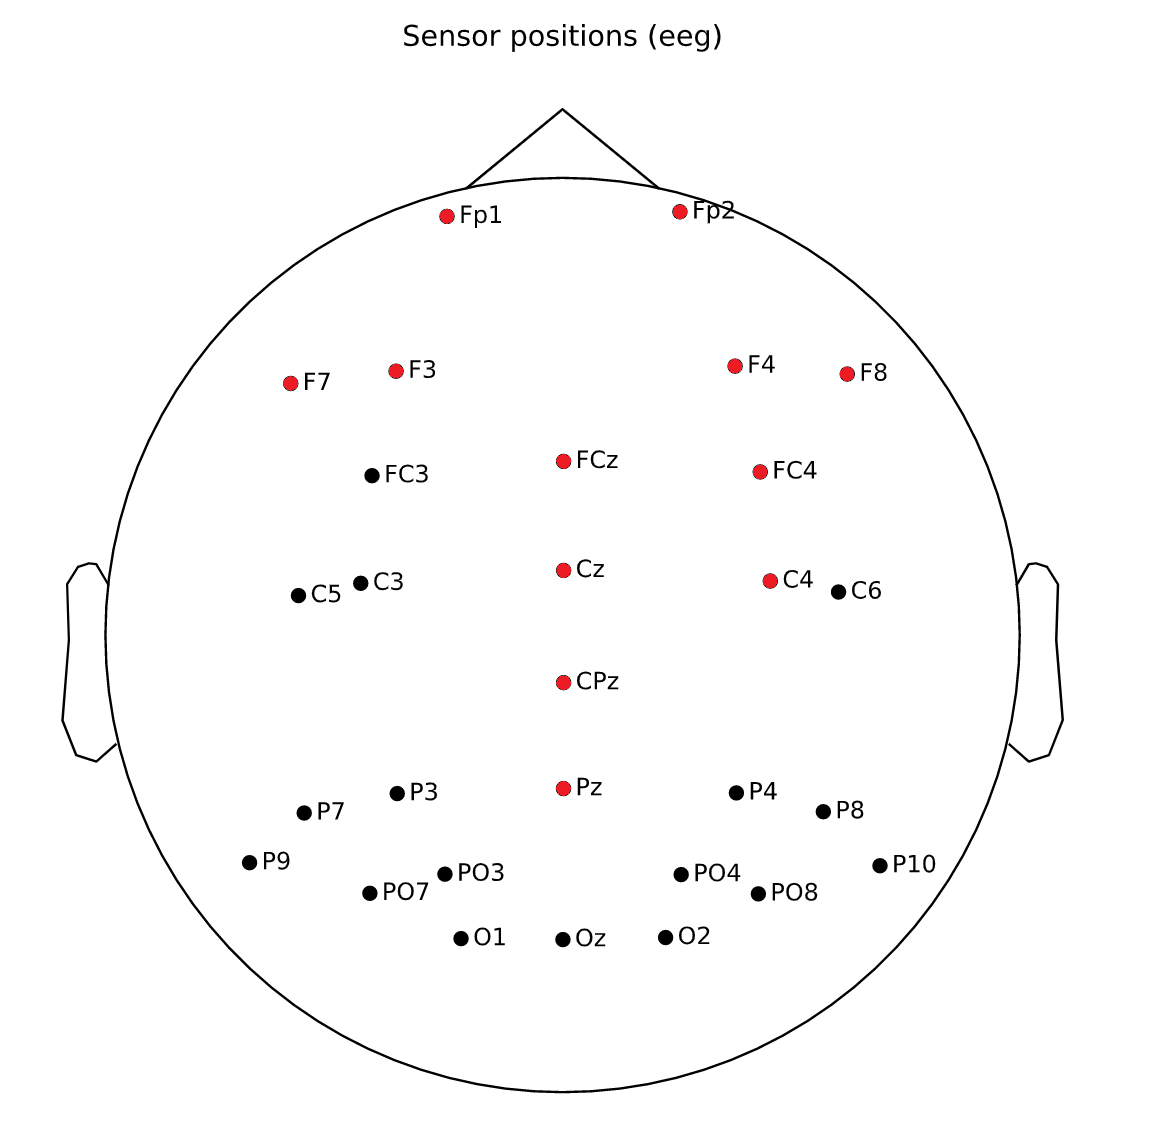
\includegraphics[width=0.7\textwidth]{effectChannels.png}
  \caption{Location of electrodes marked in red for which the t-test between target and distractor stimulus groups showed a significant effect with a p-value of $p \leq 0.05$.}
  \label{fig:effectChannels}
\end{figure}

\begin{figure}[tbh!] 
  \centering
     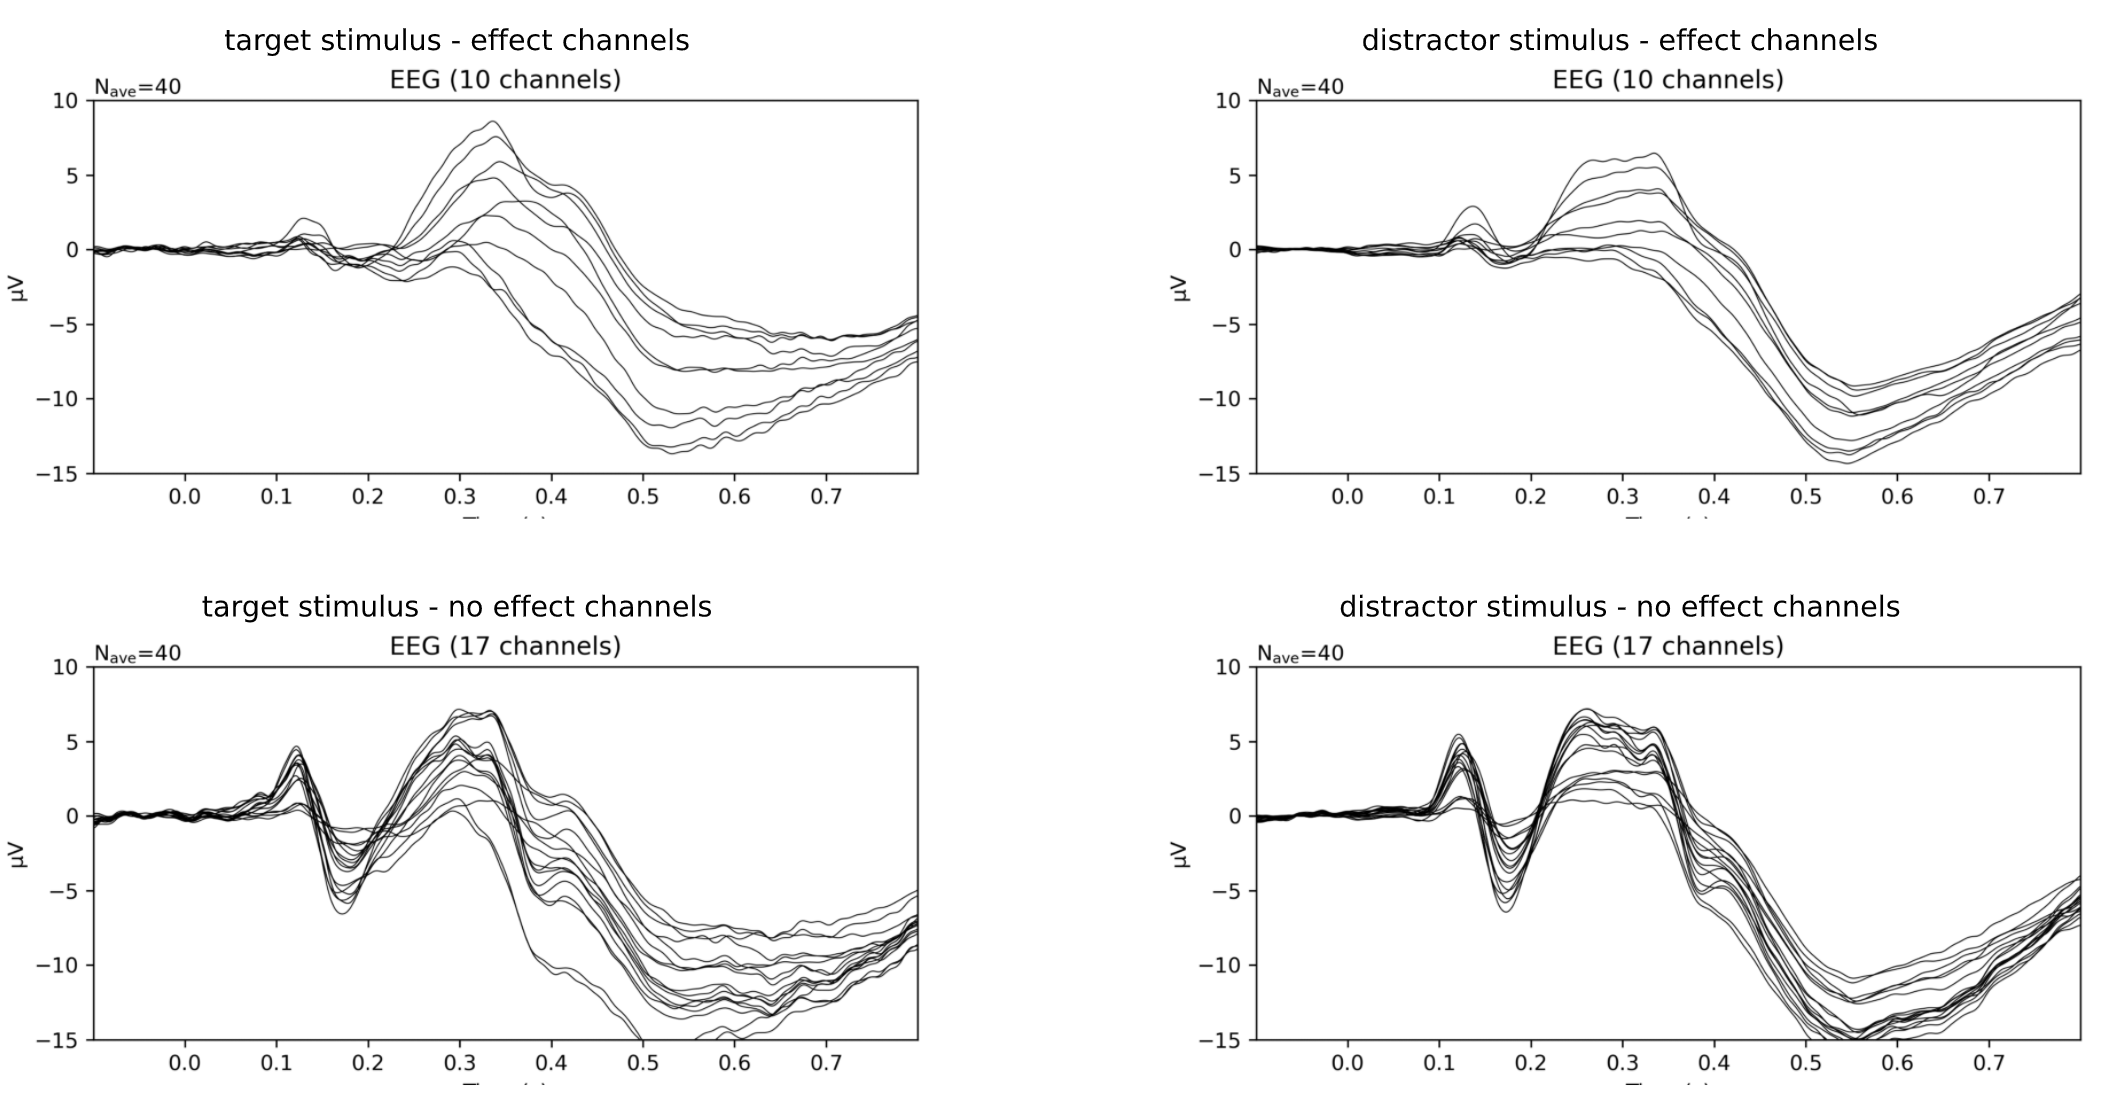
\includegraphics[width=1.1\textwidth]{erpGrandAverage.png}
  \caption{ERP grand averages of effect channels and channels without effect, grouped by the presence of target stimulus for all subjects $n=40$.}
  \label{fig:erpGrandAverage}
\end{figure}
\FloatBarrier
%~\ref{tab:ttest}
The t-test tests the groups target and distractor for differences in their peak values caused by their conditions.
The scipy.stats.ttest Python module is used to perform the test.
The results of the t-test are shown in table 3, which shows $\sigma < 0.05$ for 12 different channels (FCz, F4, F7, Cz, F3, F8, CPz, FC4, FP2, Pz, FP1, C4).
The electrodes of these channels are all located in the parieto-central area of the brain as shown in figure~\ref{fig:effectChannels}.
\caay{picton1992} also found a similar effect in the parieto-central area known as the P300 wave for subjects actively engaged in the task of detecting a target stimulus. 

After identifying the channels with a significant effect of the target stimulus condition, grand average ERPs can be created for all subjects.
For all subjects $n=40$, four grand average ERPs are plotted in figure~\ref{fig:erpGrandAverage}.
This allows for comparison of the grand average ERPs for channels with and without significant effect of the peak value while respecting their class membership to target and distractor.
In general effect channels show a higher total amplitude and a prolonged effect of many channels reaching the -5\textmu v after 500ms.
These effect channels reach the -5\textmu v mark before 500ms if a distractor stimulus is shown.
On the bottom of figure~\ref{fig:erpGrandAverage} the channels without signifcant effect of stimulus condition are compared,  which are more similar than the upper grand average ERPs.
The results of the ERP peak value t-test and the grand average ERP plots of the channels with effect confirm that there is a significant difference in 12 channels in the parieto-central region when subjects are exposed to the targets stimulus.

\section{Mass univariate analysis}
\label{sec:massuni}
In this section a multiple regression is fitted to the values of the channels with a significant effect identified in section~\ref{sec:erp}.
The experiment with subject $S_2$ is used for fitting, using the predictor variables reaction time and stimulus condition.
For each epoch ($n=200$, $n_{target}=40$, $n_{distractor}=160$) the reaction time is computed by subtracting the time of the stimulus onset from the time of the answer event onset.
Distractor stimulus events are encoded with the numerical value 1 and the target events are encoded with the value 2 (see figure~\ref{fig:mrEvents}).
The reaction time is stored in seconds in a pandas data frame, along with the other predictor variables.

\begin{figure}[tbh!] 
  \centering
     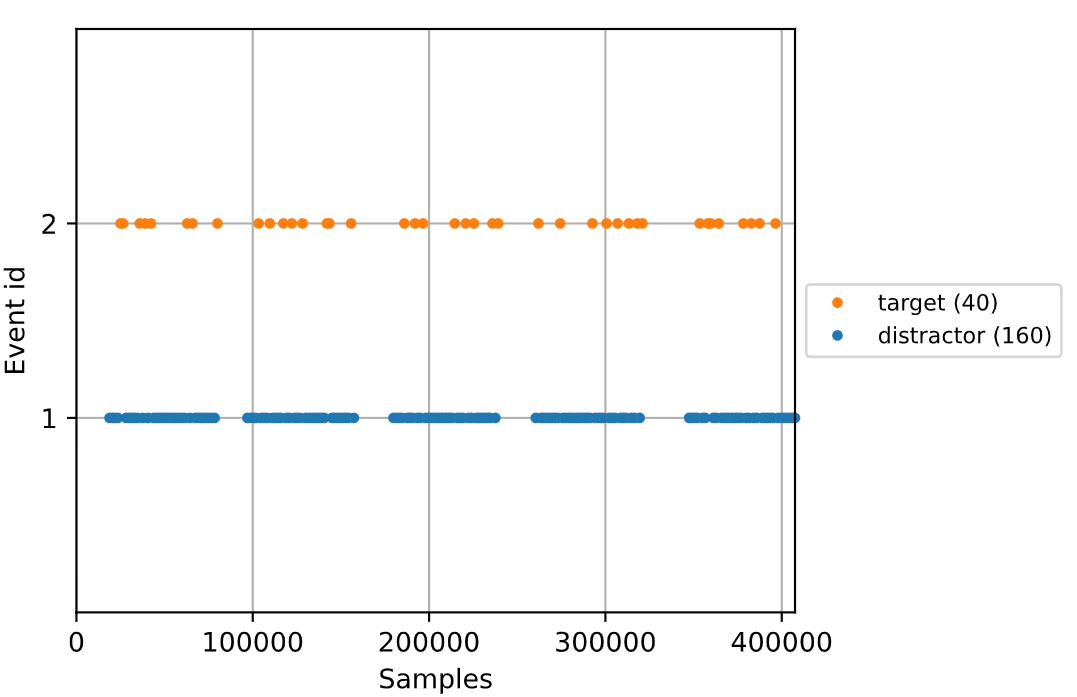
\includegraphics[width=0.5\textwidth]{mrEvents.png}
  \caption{Distribution of events for $S_2$}
  \label{fig:mrEvents}
\end{figure}

\begin{figure}[tbh!] 
  \centering
     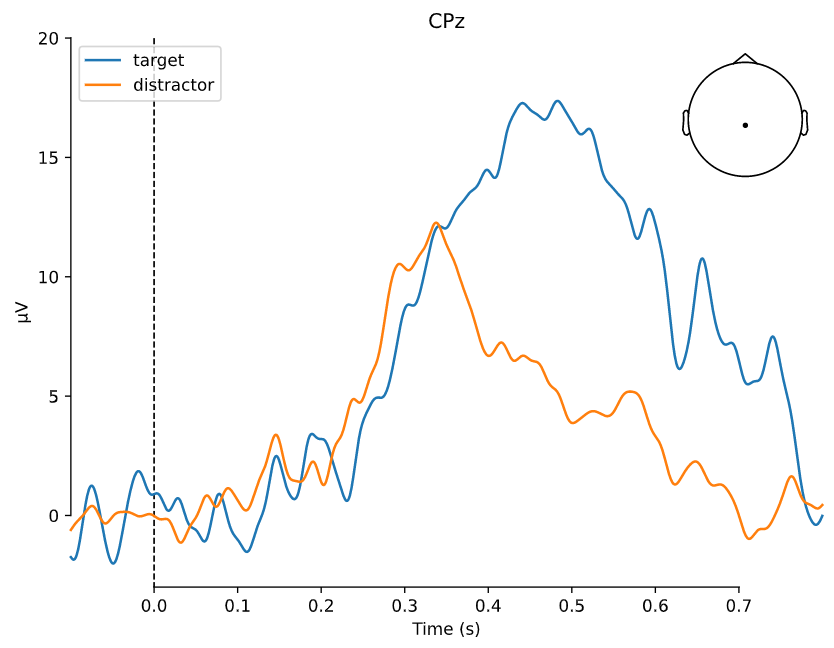
\includegraphics[width=0.7\textwidth]{mrCompEvokeds.png}
  \caption{Comparison of target and distractor evokeds for $S_2$ for $n=200$ epochs for the channel Cz.}
  \label{fig:mrCompEvokeds}
\end{figure}


\begin{comment}
\begin{figure}[tbh!] 
\centering
 \begin{subfigure}[t]{0.5\textwidth}
        \centering
        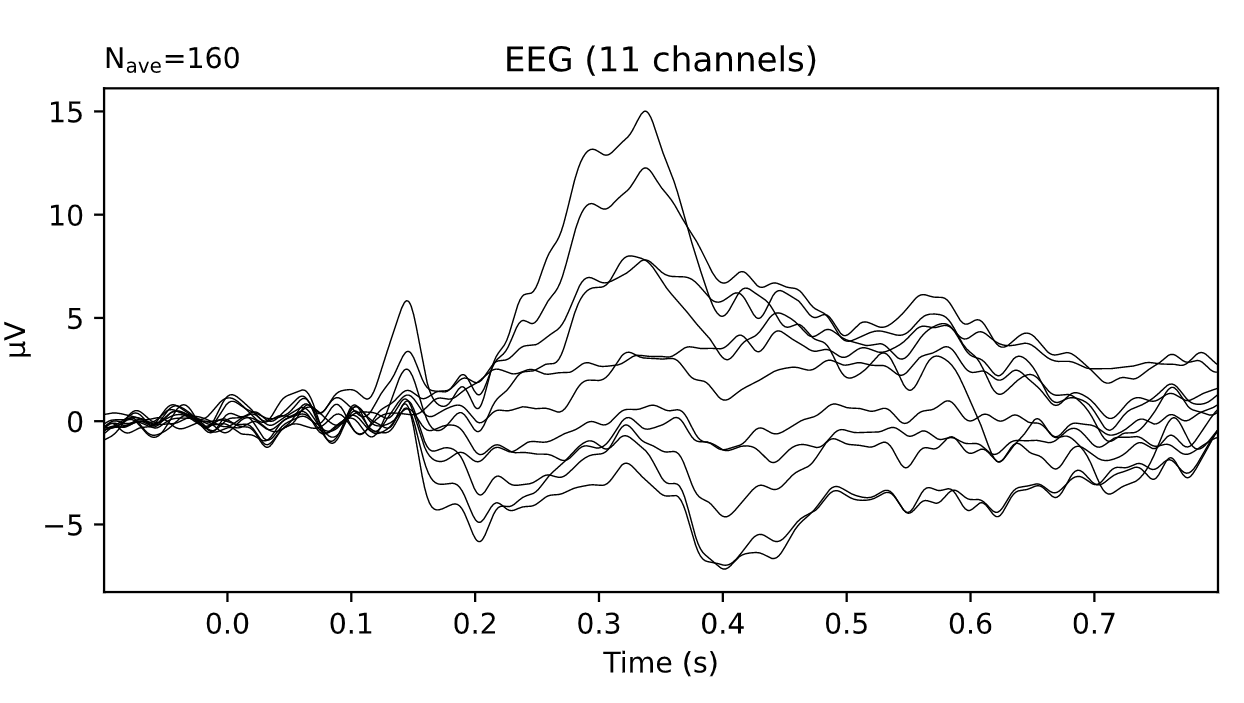
\includegraphics[height=1.3in]{mrDistractor.png}
	\caption{ERP averages of $S_2$ for 160 distractor epochs for all channels with effect.}
\end{subfigure}%
    ~ 
\begin{subfigure}[t]{0.5\textwidth}
        \centering
        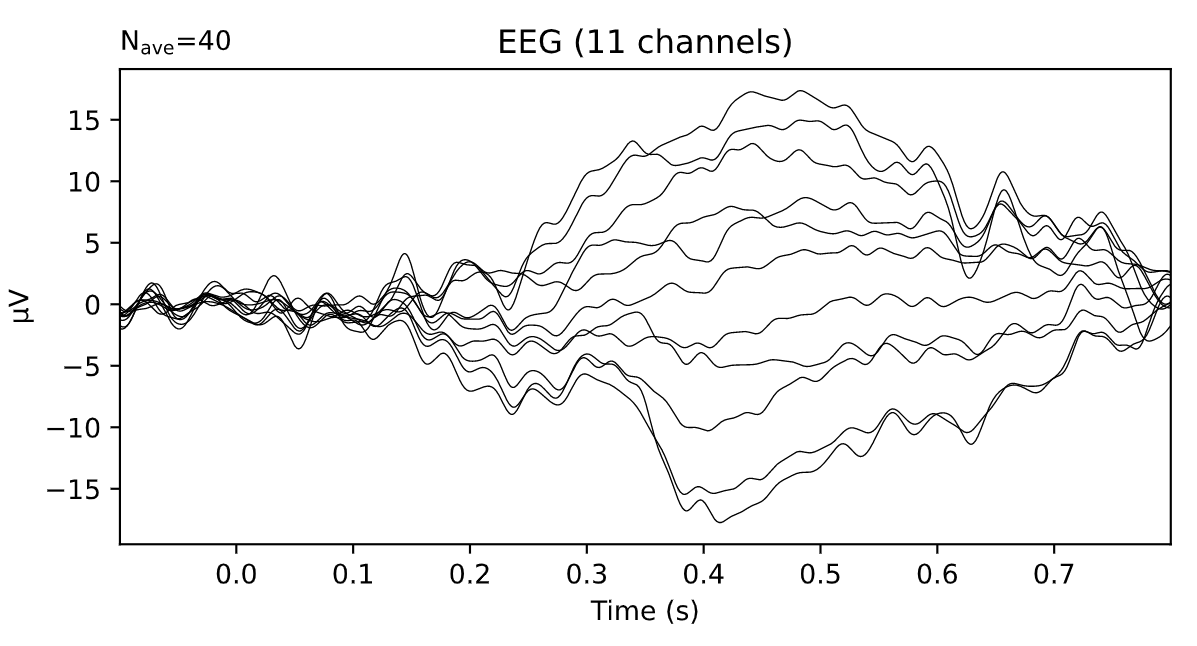
\includegraphics[height=1.3in]{mrTarget.png}
        \caption{ERP averages of $S_2$ for 40 target epochs for all channels with effect.}
\end{subfigure}
     \label{fig:mrComp}
\end{figure}
\end{comment}

\FloatBarrier
With the extracted data of the reaction time a first plot showcasing the influence of the reaction time on channel amplitude can be generated using the mne.plot\textunderscore compare\textunderscore evokeds() method (fig.~\ref{fig:mrReactionTimeEffect}).
However, from this plot it does not seem that the EEG signal is in any way correlated to the reaction time.

\begin{figure}[tbh!] 
  \centering
     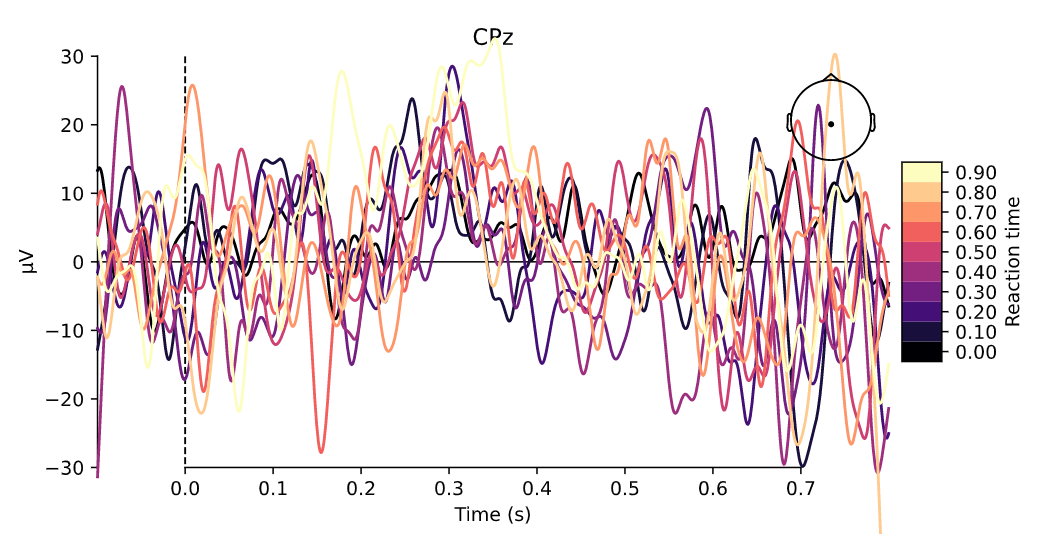
\includegraphics[width=0.7\textwidth]{mrReactionTimeEffect.png}
  \caption{Evokeds of $S_2$ with their reaction time mapped to color.}
  \label{fig:mrReactionTimeEffect}
\end{figure}

Finally the design matrix for the multiple regression incorporates:
\begin{itemize}
\item stimulus as categoriocal variable (distractor =1, target = 2)
\item answer as categorical variable (incorrect = 1, correct = 2)
\item reaction time as continous variable
\item intercept = 1
\end{itemize}

The channel data for 11 channels for 922 timepoints with effect is fitted using the design matrix, resulting in 10142 targets and the 4 regressors.
To fit the data, the Python module mne.stats.linear\textunderscore regression is used.
After the fit is done, the beta values of the reaction time can be plotted in a butterfly plot (see fig.~\ref{fig:mrBetaRT}).
A very small effect of the reaction time starting at 400ms can be identified.

\begin{figure}[tbh!] 
  \centering
     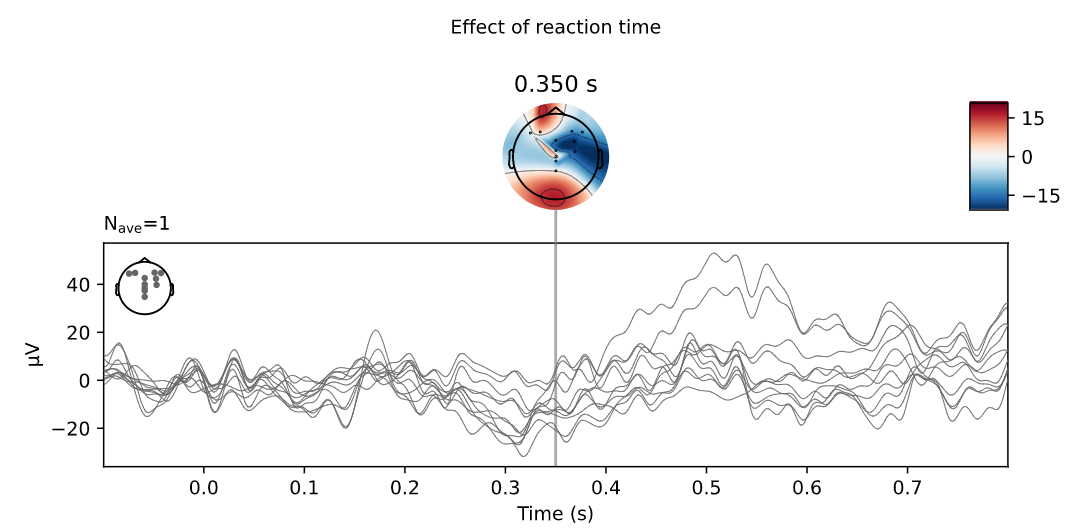
\includegraphics[width=0.7\textwidth]{mrBetaRT.png}
  \caption{beta values of the reaction time feature}
  \label{fig:mrBetaRT}
\end{figure}

\begin{figure}[tbh!] 
  \centering
     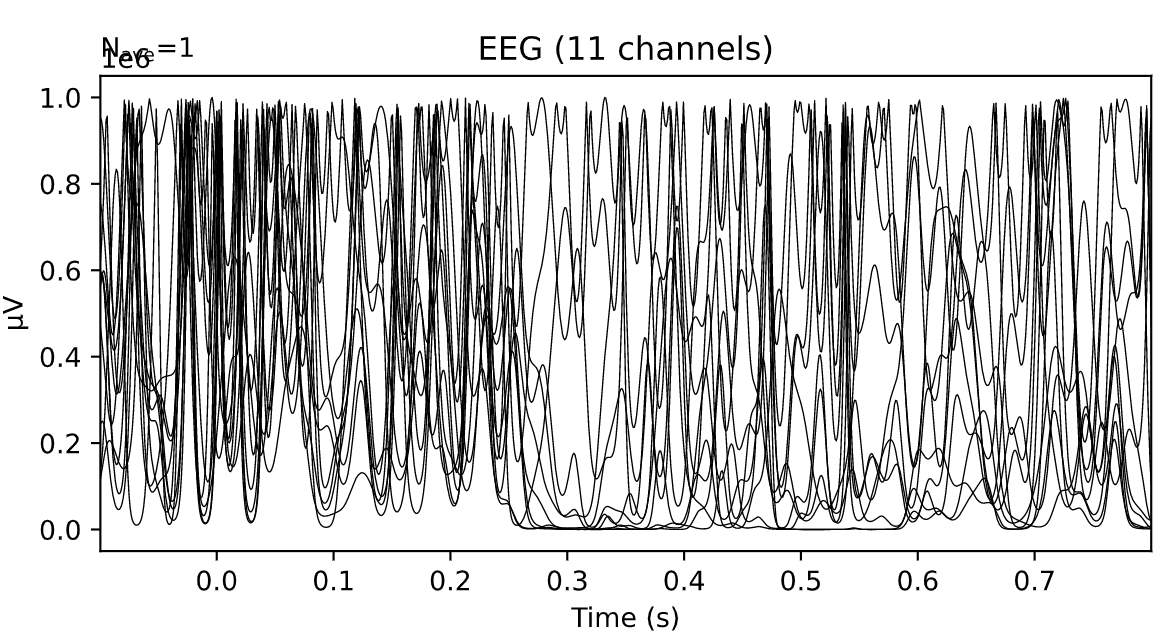
\includegraphics[width=0.7\textwidth]{mrPval.png}
  \caption{p values of the reaction time feature}
  \label{fig:mrPval.png}
\end{figure}


\section{Decoding over time}
\label{sec:decoding}
Decoding in the context of EEG aims at predicting experiment conditions such as a stimulus condition shown to the subject using the EEG channel data.
For this decoding analysis, a machine learning model is trained to classify a point in time of unknown condition into the classes \textit{target} and \textit{distractor} depending on which stimulus was shown to the subject.
This is a binary classification problem, so the base rate for correct classification by using random assignment is already at $p=0.5$.
A sliding window solves the classification problem for each time step in the epoch.
If there are significant effects correlated to experiment stimuli at certain points in time, the binary classifier will perform better at these points in time.
If at certain time intervals no correlation of EEG data and experiment stimulus is present, the binary classifier will achieve the base rate accuracy close to $p=0.5$.

\subsection{Decoding on all subjects}
The data used for training includes all 40 subjects and all shared good channels.
If for some subject a channel is declared as bad, this channel is not used for all subjects.
The EOG channels HEOG right and left and VEOG\textunderscore lower are excluded.
Finally, 28 EEG channels are used for training.
In total there are 7135 epochs from all subjects, with 1443 epochs of class \textit{target} and 5692 \textit{distractor} epochs (see fig.~\ref{fig:decodeComp}).
The predictor data $X$ is retrieved from the epochs using the mne method epochs.get\textunderscore data().
The class labels $Y$ are extracted from epochs.events with \textit{distractor}=1 and \textit{target}=2.
The StandardScaler() from sklearn.preprocessing is used for scaling the data.
To fit the data at each timepoint of the epochs the SlidingEstimator from mne.decoding module is used.
Classification is scored using the ROC AUC (receiver operating characteristics - area under the curve) score.
The ROC AUC is plotted with the false positive rate on the x-axis and the true positive rate on the y-axis.
The ROC is the curve characteristic of this curve, ideally it is a square with area under the curve $AUC=1$.
If the classifier in a binary classification problem has an accuracy of $p=0.5$ the ROC curve is the linear function $f(x) =x$, resulting in $AUC=0.5$.
If the distributions of classifications overlap the ROC characteristic takes the form of a non-linear function.
Using the mne method cross\textunderscore val\textunderscore multiscore() the model is trained with $X$ and $Y$ as input using a 5-fold cross validation.

\begin{figure}[tbh!] 
\centering
 \begin{subfigure}[t]{0.5\textwidth}
        \centering
        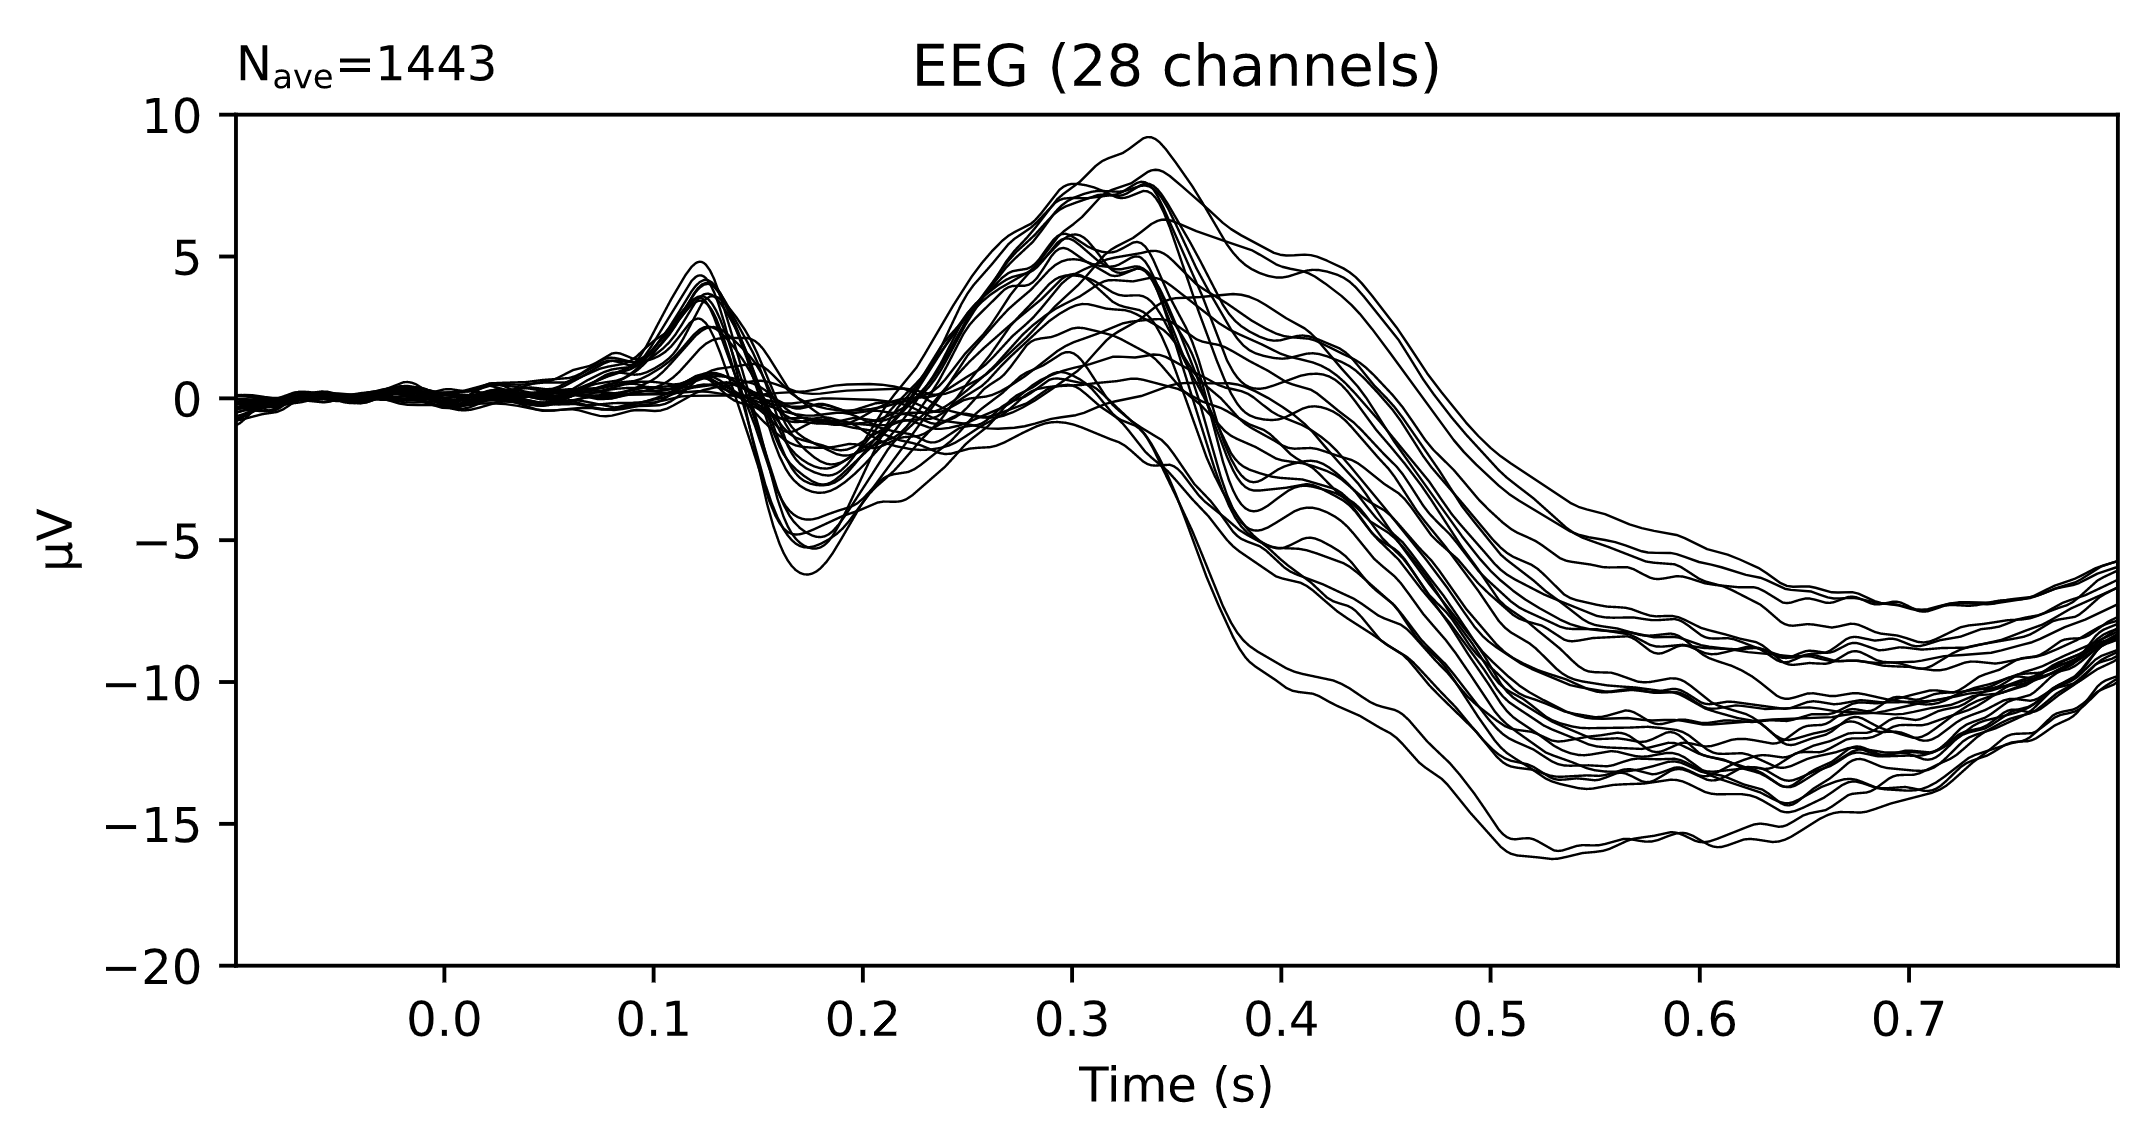
\includegraphics[height=1.5in]{decodingTarget.png}
\end{subfigure}%
    ~ 
\begin{subfigure}[t]{0.5\textwidth}
        \centering
        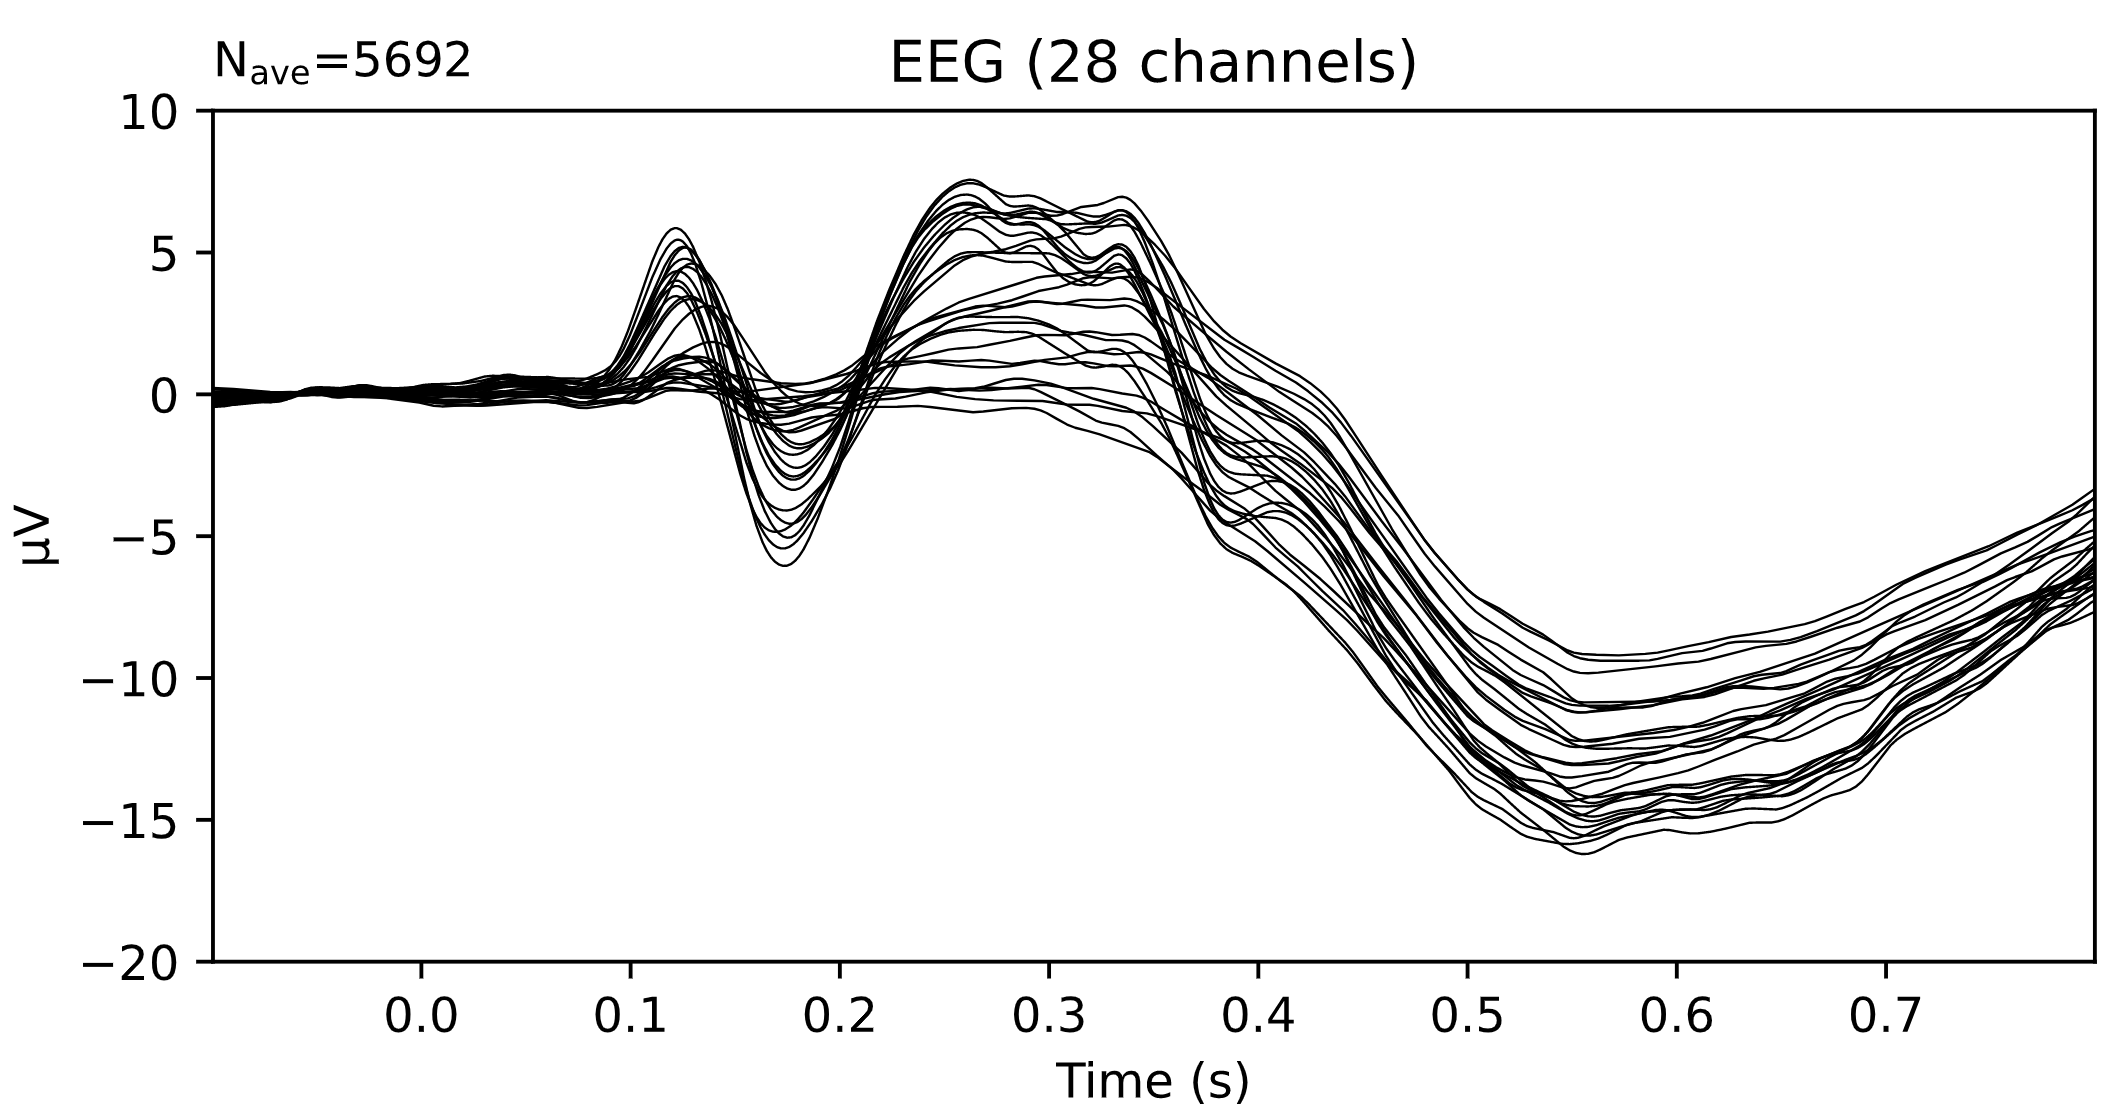
\includegraphics[height=1.5in]{decodingDistractor.png}
\end{subfigure}
	\caption{ERP averages of 28 channels used for decoding from all 40 subjects from epochs with target (left) and distractor (right) stimulus.}
     \label{fig:decodeComp}
\end{figure}

After the training process finished, the scores of each cross-validation run are averaged and plotted over time.
Figure~\ref{fig:decodingScore} shows the decoding results.
Obviously the classifier is unable to predict better than chance before $t=0.2s$ as the score in this interval is very close to the base rate probability.
A significant effect starts after $t=0.2s$ and lasts until $t=0.6s$ as the ROC AUC increases to 0.65.
At first sight the peak scores of the classifier seem rather low with 0.65 in a binary classification problem.
However, this is probably caused by using epoch data from all subjects which all exhibit different peak amplitude values for the target and distractor stimuli.
As each subject is different, peak distractor stimuli epoch values can match another subjects peak target stimuli epoch exacerbating the classification process.
In further research the classifier score may be improved by normalizing the channels of each subject to a common value range.

\begin{figure}[tbh!] 
  \centering
     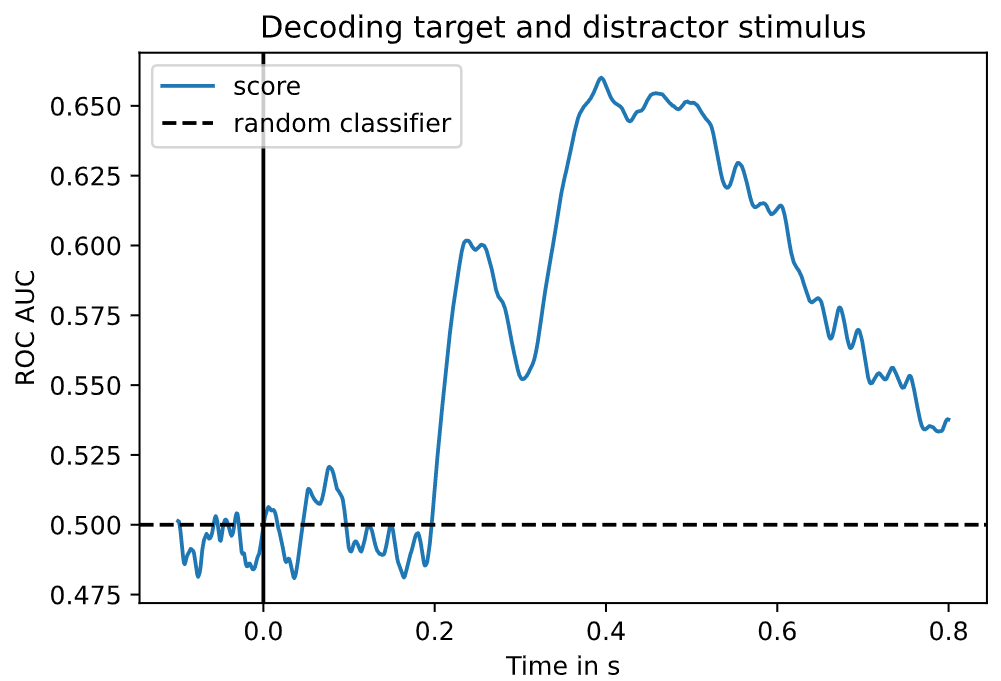
\includegraphics[width=0.7\textwidth]{decodingScore.png}
  \caption{Score of the binary classifier trained with $n=7135$ epochs over time.}
  \label{fig:decodingScore}
\end{figure}

\subsection{Decoding on a single subject}
To test the theory of the cause of low ROC AUC scores for all epochs due to different subjects, the same decoding procedure is repeated using only training data from a single subject.
All epochs of 30 EEG Channels of subject $S_2$ are used for training with 40 target stimulus epochs and 160 distractor stimulus epochs.
The results of this single subject decoding can be seen in figure~\ref{fig:decodingScoreS2}.
Before $t=0.2$ the score is close to the random classifier, no significant effect of the target stimulus can be used by the classifier.
Starting at $t=0.2$ the score increases.
The most prominent interval with high classification score is between $t=0.3$ and $t=0.6$.
In this interval the area under the curve is greater than 0.8 indicating a significant effect of the target stimulus after 300ms.
The effect starts to vanish after $t=0.6$ and probably will reach a score close to 0.5 again shortly after $t=0.8$.
\begin{figure}[tbh!] 
  \centering
     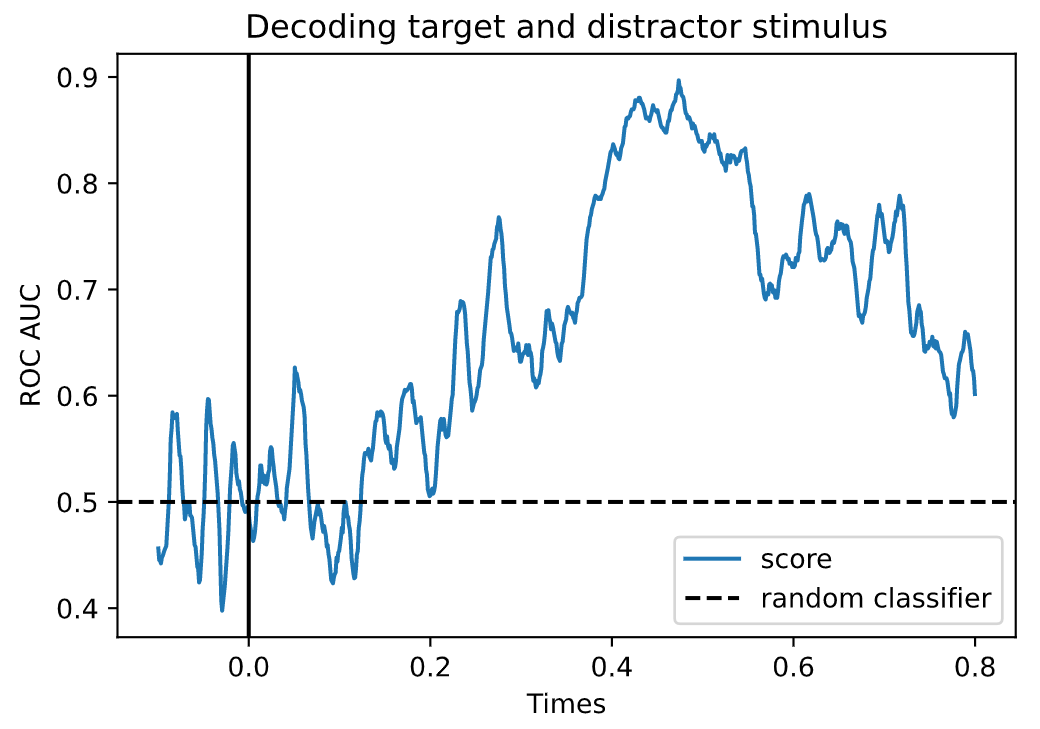
\includegraphics[width=0.7\textwidth]{decodingScoreS2.png}
  \caption{Score of the binary classifier trained on 200 epochs of subject $S_2$.}
  \label{fig:decodingScoreS2}
\end{figure}

In conclusion a significant effect of the target stimulus after 300ms could be shown for all subjects as well as a single subject.
This confirms the results of \caay{Kappenman2021}, who also detected the P300 prolonged effect when the brain is trying to detect a target amid distractor stimuli.

\newpage
\pagenumbering{roman}


\FloatBarrier
\section{Declaration of authorship}
% freigabeklausel + unterschrift pascal kuhn + unterschrift marcel hasenbalg
I hereby declare that the report submitted is my own unaided work. 
All direct or indirect sources used are acknowledged as references.
I am aware that the report in digital form can be examined for the use of unauthorized aid and in order to determine whether the thesis as a whole or parts incorporated in it may be deemed as plagiarism. 
For the comparison of my work with existing sources I agree that it shall be entered in a database where it shall also remain after examination, to enable comparison with future theses submitted.
	\begin{flushleft}
    	
\includegraphics[width=2in]{signature} % adjust width as necessary or use scale
	\end{flushleft}
\newpage
\printbibliography
\end{document}